\documentclass[C++.tex]{subfiles}
\begin{document}

\section{C++11}
\subsection*{Présentation}
\begin{frame}
	\frametitle{Présentation}
	\begin{itemize}
		\item Approuvé unanimement le 12 août 2011
	
\note[item]{Formellement, C++11 remplace C++03 et a été remplacé par C++14}
	
		\item Dernier \textit{Working Draft} : \href{http://www.open-std.org/jtc1/sc22/wg21/docs/papers/2012/n3337.pdf}{N3337}
	
\note[item]{Différences entre le standard et ce draft : des corrections éditoriales}
	
		\item Standardisation laborieuse
		\begin{itemize}
			\item Sortie tardive (C++0x)
			\item Périmètre initial trop ambitieux (retrait des concepts en 2009)
		\end{itemize}
		\item Changement de fonctionnement du comité
		\begin{itemize}
			\item Utilisation de \textit{Technical Specification} et de groupes de travail dédiés
			\item Pilotage par les dates plutôt que par les fonctionnalités (\textit{train model})
			\item Des versions fréquentes (3 ans : 2011, 2014, 2017, 2020, \ldots)
			\item Voir \href{https://herbsutter.com/2016/03/11/trip-report-winter-iso-c-standards-meeting/}{Trip report: Winter ISO C++ standards meeting}
		\end{itemize}
		\item Très bon support par les versions récentes de GCC, Clang et VC++

\note[item]{Et de quasi tout les compilateurs, à l'exception de Digital Mars}

		\item Objectifs : plus sûr, plus simple, aussi rapide que possible, meilleure détection d'erreur au compile-time
	
\note[item]{Plus sûr : type-safe et resource-safe - meilleur typage, RAII, etc.}
\note[item]{Plus simple : vu comme un langage \og pour expert \fg{}, volonté d'être plus \textit{beginner friendly}, plus facile à apprendre, à enseigner et à utiliser}
\note[item]{Aussi rapide : conserve le \og ne pas payer pour ce que l'on utilise pas\fg{}}
\note[item]{Compilation : meilleure détection d'erreur rejoint en partie le plus sûr, diagnostique plus clair}

\note[item]{Pas complet, je laisse de côté \lstinline|system_error|, \lstinline|codecvt|, \lstinline|typeindex| et deux-trois nouvelles fonctions dans la bibliothèque standard}
	\end{itemize}
\end{frame}

\subsection*{Nouveaux types}
\begin{frame}[fragile]
	\frametitle{Nouveaux types entiers\titlehfill{}1/3}
	\begin{itemize}
		\item Hérités de C99 (\lstinline[keywordstyle=\color{black}]|cstdint| et \lstinline|cinttypes|)
	\end{itemize}

	\begin{block}{Intégration depuis C99}
		Outre les nouveaux types : \textit{variadic macro}, \lstinline|__func__|, concaténation de chaînes littérales, \ldots

\note[item]{En pratique déjà supportés par certains compilateurs sous forme d'extensions}
	\end{block}

	\begin{itemize}
		\item \lstinline|long long int| et \lstinline|unsigned long long int|
		\begin{itemize}
			\item Au moins aussi grand que \lstinline|long int|
			\item Plages garanties : [$-(2^{63}-1)$, $2^{63}-1$] et [$0$, $2^{64}$]
			\item Extension de nombreux compilateurs bien avant C++11
		\end{itemize}
		\item \lstinline|intmax_t| et \lstinline|uintmax_t| : types entiers le plus grand disponibles
	\end{itemize}
\end{frame}

\begin{frame}[fragile]
	\frametitle{Nouveaux types entiers\titlehfill{}2/3}
	\begin{itemize}
		\item \lstinline|int<N>_t| et \lstinline|uint<N>_t| : types entiers de N bits
		\begin{itemize}
			\item N = 8, 16, 32 ou 64
			\item Types signés obligatoirement en complément à 2

\note[item]{En C++, pas de contrainte sur les autres types entiers signés}
\note[item]{En C, d'autres représentations possibles : signe + valeur (avec deux codages de 0, algorithme d'addition/ multiplication non canonique) et complément à 1 où chaque bit du positif est inversé pour donner le négatif, là encore deux valeurs de 0}
\note[item]{Complément à 2 : inversion de chaque bit (complément à 1) puis ajout de 1}

			\item Pas de bit de \textit{padding}
			\item Optionnels (uniquement si un type compatible existe)
		\end{itemize}
		\item \lstinline|int_least<N>_t| et \lstinline|uint_least<N>_t| : plus petits types entiers d'au moins N (8, 16, 32 ou 64) bits
		\item \lstinline|int_fast<N>_t| et \lstinline|uint_fast<N>_t| : plus rapides types entiers d'au moins N (8, 16, 32 ou 64) bits
		\item \lstinline|intptr_t| et \lstinline|uintptr_t| : type entier capable de contenir une adresse
		\begin{itemize}
			\item Doit pouvoir être reconvertit en \lstinline|void*| avec une valeur égale au pointeur original
			\item Optionnels
		\end{itemize}
	\end{itemize}
\end{frame}

\begin{frame}[fragile]
	\frametitle{Nouveaux types entiers\titlehfill{}3/3}
	\begin{itemize}
		\item Macros de définition des plages correspondantes
		\item Macros de construction depuis des entiers \og classiques\fg{}
		\item Macros des spécificateurs pour \lstinline|printf| et \lstinline|scanf|
		\item Fonctions de manipulation de \lstinline|intmax_t| et \lstinline|uintmax_t| (\lstinline|imaxabs|, \lstinline|imaxdiv|, \lstinline|strtoimax|, \lstinline|strtoumax|, \lstinline|wcstrtoimax| et \lstinline|wcstrtoumax|)
		\item Surcharges de \lstinline|abs| et \lstinline|div| pour \lstinline|intmax_t| si nécessaire

\note[item]{Si nécessaire, c'est à dire si ce n'est pas un alias sur un autre type fondamental}
	\end{itemize}
\end{frame}

\begin{frame}[fragile]
	\frametitle{POD Généralisé - Rappels}
	\begin{itemize}
		\item Types POD (\textit{Plain Old Data}) : classes et structures POD, unions POD, types scalaires et tableaux de ces types
		\item Certaines constructions ne sont permises que pour les types POD

\note[item]{Permises \textbf{uniquement} sur les POD vue de la norme tout du moins. En pratique, certaines opérations peuvent fonctionner sur des types non-POD sur une implémentation particulière}

		\begin{itemize}
			\item Utilisation de \lstinline|memcpy()| ou \lstinline|memmove()|
			\item Utilisation de \lstinline|goto| \og au-dessus\fg{} de la déclaration d'une variable

\note[item]{C'est à dire depuis un point où la variable n'est pas dans le scope vers un point où la variable est déjà dans le scope}

			\item Utilisation de \lstinline|reinterpret_cast|
			\item Accès au début commun d'une union par un membre non actif
			\item Utilisation des fonctions C \lstinline|qsort()| ou \lstinline|bsearch()|
			\item \ldots
		\end{itemize}
	\end{itemize}
\end{frame}

\begin{frame}[fragile]
	\frametitle{POD Généralisé - Classe agrégat}
	\begin{itemize}
		\item C++98
		\begin{itemize}
			\item Pas de constructeur déclaré par l'utilisateur
			\item Pas de donnée membre non-statique privée ou protégée
			\item Pas de classe de base
			\item Pas de fonction virtuelle
		\end{itemize}
		\item C++11
		\begin{itemize}
			\item Pas de constructeur \underline{fourni} par l'utilisateur

\note[item]{Les constructeurs déclarés \lstinline|=default| par l'utilisateur sont autorisés}

			\item Pas d'initialisation \textit{brace-or-equal-initializers} des données membres non-statiques
			\item Pas de donnée membre non-statique privée ou protégée
			\item Pas de classe de base
			\item Pas de fonction virtuelle
		\end{itemize}
	\end{itemize}

	\begin{block}{En C++14}
		Suppression de la contrainte \og Pas d'initialisation \textit{brace-or-equal-initializers} des données membres non-statiques\fg{}
	\end{block}
\end{frame}

\begin{frame}[fragile]
	\frametitle{POD Généralisé - Classe POD C++98}
	\begin{itemize}
		\item Classe agrégat
		\item Pas de donnée membre non-statique de type non-POD (ou de tableau de non-POD) ni de référence
		\item Pas d'opérateur d'assignation défini par l'utilisateur
		\item Pas de destructeur défini par l'utilisateur
	\end{itemize}
\end{frame}

\begin{frame}[fragile]
	\frametitle{POD Généralisé - Classe POD C++11\titlehfill{}1/4}
	\begin{itemize}
		\item Contraintes réparties en trois sous-notions
		\item \textit{trivially copyable}
		\begin{itemize}
			\item Pas de constructeur de copie ou de déplacement non triviaux
			\item Pas d'opérateur d'affectation non trivial
			\item Destructeur trivial
		\end{itemize}
	\end{itemize}

	\pause

	\begin{block}{Trivial ?}
		\begin{itemize}
			\item Pas fournie par l'utilisateur
			\item Pas de fonction virtuelle ni de classe de base virtuelle
			\item Opération des classes de bases et des membres non-statiques est triviale
		\end{itemize}
	\end{block}

	\pause

	\begin{block}{Autre formulation}
		\begin{itemize}
			\item Copie, déplacement, affectation et destruction générés implicitement
			\item Pas de fonction ni de classe de base virtuelle
			\item Classes de base et membres non-statiques \textit{trivially copyable}
		\end{itemize}
	\end{block}
\end{frame}

\begin{frame}[fragile]
	\frametitle{POD Généralisé - Classe POD C++11\titlehfill{}2/4}
	\begin{itemize}
		\item \textit{trivial}
		\begin{itemize}
			\item \textit{trivially copyable}
			\item Constructeur par défaut trivial
			\begin{itemize}
				\item Pas fourni par l'utilisateur
				\item Pas de fonction virtuelle ni de classe de base virtuelle
				\item Constructeur par défaut des classes de base et des membres non-statiques trivial
				\item Pas d'initialisation \textit{brace-or-equal-initializers} des données membres non-statiques
			\end{itemize}
		\end{itemize}
	\end{itemize}
\end{frame}

\begin{frame}[fragile]
	\frametitle{POD Généralisé - Classe POD C++11\titlehfill{}3/4}
	\begin{itemize}
		\item \textit{Standard-layout}
		\begin{itemize}
			\item Pas de donnée membre non-statique non-\textit{Standard-layout} ni de référence
			\item Pas de classe de base non-\textit{Standard-layout}
			\item Pas de fonction virtuelle ni de classe de base virtuelle
			\item Même accessibilité de toutes les données membres non-statique
			\item Données membres non-statiques localisées dans une unique classe de l'arbre d'héritage

\note[item]{Formellement : pas de données membres non-statiques dans la classe la plus dérivée et au plus une classe de base avec des données membres non-statiques ou pas de clase de base avec des données membres non-statiques}

			\item Pas de classe de base du type de la première donnée membre non-statique

			\begin{block}{En résumé}
				Organisation mémoire similaire aux structures C
			\end{block}
		\end{itemize}
	\end{itemize}
\end{frame}

\begin{frame}[fragile]
	\frametitle{POD Généralisé - Classe POD C++11\titlehfill{}4/4}
	\begin{itemize}
		\item POD
		\begin{itemize}
			\item \textit{trivial}
			\item \textit{standard layout}
			\item Pas de donnée membre non-statique non-POD
		\end{itemize}
		\item Ajout des traits correspondants : \lstinline|std::is_trivial|, \lstinline|std::is_trivially_copyable| et \lstinline|std::is_standard_layout|
	\end{itemize}
\end{frame}

\begin{frame}[fragile]
	\frametitle{POD Généralisé - Objectifs}
	\begin{itemize}
		\item Opérations réservées au POD deviennent accessibles aux classes de la sous-notion correspondante
		\item Relâchement / adaptation de certaines contraintes par rapport
		\begin{itemize}
			\item Constructeurs ou destructeurs déclarés \lstinline|=default| autorisés
			\item Données membres non-statiques ne sont plus nécessairement publiques

\note[item]{Mais doivent toutes avoir la même portée, ceci vient du fait qu'en C++, le compilateur peut réordonner les données de portées différentes}

			\item Classes de base non virtuelles autorisées

\note[item]{A condition de respecter les contraintes de type et de localité des données membre}
		\end{itemize}
	\end{itemize}
\end{frame}

\begin{frame}[fragile]
	\frametitle{POD Généralisé - Quelques conséquences}
	\begin{itemize}
		\item \textit{standard layout}
		\begin{itemize}
			\item Utilisation de \lstinline|reinterpret_cast|
			\item Accès au début commun d'une union par un membre non actif
			\item Usage de \lstinline|offsetof|
		\end{itemize}
	
		\item \textit{trivially copyable}
		\begin{itemize}
			\item Utilisation de \lstinline|memcpy()| ou \lstinline|memmove()|
		\end{itemize}

		\item \textit{trivial}
		\begin{itemize}
			\item Utilisation de \lstinline|goto| \og au-dessus\fg{} de la déclaration d'une variable
			\item Utilisation des fonctions C \lstinline|qsort()| ou \lstinline|bsearch()|
		\end{itemize}
	\end{itemize}
\end{frame}

\begin{frame}[fragile]
	\frametitle{Unions généralisées}
	\begin{itemize}
		\item Types avec des constructeurs, opérateurs d'assignation ou destructeurs définis par l'utilisateur acceptés comme membre d'une union
		\item \ldots mais les fonctions équivalentes de l'union sont supprimées

\note[item]{Il est donc impossible de copier une union si un des membres est un type possédant un constructeur de copie défini par l'utilisateur. Ce qui limite, à mon avis, un peu l'intérêt}

		\item Toujours impossible d'utiliser des types avec des fonctions virtuelles, des références ou des classes de base
	\end{itemize}
\end{frame}

\subsection*{namespace}
\begin{frame}[fragile]
	\frametitle{inline namespace}
	\begin{itemize}
		\item Injection des déclarations du namespace imbriqué dans le namespace parent
	\end{itemize}

	\begin{lstlisting}[language=C++]
namespace V1 { void foo() { cout << "V1\n"; } }

inline namespace V2 { void foo() { cout << "V2\n"; } }

V1::foo();  // Affiche V1
V2::foo();  // Affiche V2
foo();      // Affiche V2\end{lstlisting}

	\begin{block}{Motivation}
		Évolution de bibliothèque et conservation des versions précédentes
	\end{block}
\end{frame}

\subsection*{nullptr}
\begin{frame}[fragile]
	\frametitle{\lstinline|0| ou \lstinline|NULL| ? \lstinline|nullptr| !\titlehfill{}1/2}
	\begin{itemize}
		\item C++ 98 : \lstinline|0| ou \lstinline|NULL|

\note[item]{En C++, \lstinline|NULL| est un define sur \lstinline|0| (ou équivalent), ne peut pas être \lstinline|(void*)0|}
\note[item]{\lstinline|0| ou \lstinline|NULL| : débats sans fin}

		\item Cohabite mal avec les surcharges
	\end{itemize}

	\onslide<2>
	\begin{block}{Quiz : Quelle surcharge est éligible ?}
		\begin{lstlisting}[language=C++]
void foo(char*) { cout << "chaine\n"; }
void foo(int) { cout << "entier\n"; }

foo(0);
foo(NULL);\end{lstlisting}
	\end{block}

\note[item]{GCC 8.1 en C++2a - avec \lstinline|0| :  entier, avec \lstinline|NULL| : erreur de compilation (ambiguïté)}

\end{frame}

\begin{frame}[fragile]
	\frametitle{\lstinline|0| ou \lstinline|NULL| ? \lstinline|nullptr| !\titlehfill{}2/2}
	\begin{itemize}
		\item C++ 11 : \lstinline|nullptr|
		\begin{itemize}
			\item Unique pointeur du type \lstinline|nullptr_t|
			\item Conversion implicite \lstinline|nullptr_t| vers tout type de pointeur
		\end{itemize}
	\end{itemize}

	\begin{lstlisting}[language=C++]
void foo(char*) { cout << "chaine\n"; }
void foo(int) { cout << "entier\n"; }

foo(0);        // Version int
foo(nullptr);  // Version pointeur\end{lstlisting}

	\begin{exampleblock}{Do}
		Utilisez \lstinline|nullptr| plutôt que \lstinline|0| ou \lstinline|NULL| pour désigner les pointeurs nuls
	\end{exampleblock}
\end{frame}

\subsection*{static\_assert}
\begin{frame}[fragile]
	\frametitle{\lstinline|static_assert|}
	\begin{itemize}
		\item Assertion vérifiée à la compilation
	\end{itemize}

	\begin{lstlisting}[language=C++]
static_assert(sizeof(int) == 3, "Taille incorrecte");
// Erreur de compilation indiquant "Taille incorrecte"\end{lstlisting}

	\begin{exampleblock}{Do}
		Utilisez \lstinline|static_assert| pour vérifier à la compilation ce qui peut l'être
	\end{exampleblock}

	\begin{exampleblock}{Do}
		Plus généralement, préférez les vérifications \textit{compile-time} ou \textit{link-time} aux vérifications \textit{run-time}

\note[item]{Typez correctement, définissez \lstinline|const| ce qui l'est par construction, pas de cast implicite (et donc constructeurs explicites), garantissez les invariants par construction si possible}
\note[item]{Et plusieurs autres points dans ce qui suit : opérateurs de conversion explicit, \lstinline|enum class|, \lstinline|override|, etc.}
	\end{exampleblock}
\end{frame}

\subsection*{constexpr}
\begin{frame}[fragile]
	\frametitle{\lstinline|constexpr|\titlehfill{}1/3}
	\begin{itemize}
		\item Indique une expression constante
		\item Donc évaluable et utilisable à la compilation
		\item Implicitement const

\note[item]{Plus en C++14 sur les fonctions membres}

		\item Fonctions \lstinline|constexpr| implicitement inlines
		\item Contenu des fonctions \lstinline|constexpr| limité
		\begin{itemize}
			\item \lstinline|static_assert|
			\item \lstinline|typedef|
			\item \lstinline|using|
			\item Exactement une expression \lstinline|return|
		\end{itemize}

\note[item]{Et des \textit{null statements}, mais ça n'a pas d'intérêt}
	\end{itemize}

	\begin{lstlisting}[language=C++]
constexpr int foo() {return 42;}

char bar[foo()];\end{lstlisting}
\end{frame}

\begin{frame}[fragile]
	\frametitle{\lstinline|constexpr|\titlehfill{}2/3}
	\begin{lstlisting}[language=C++]
constexpr int foo() {return 42;}

int a = 42;
switch(a)
{
  case foo():
    break;

  default:
    break;
}\end{lstlisting}
\end{frame}

\begin{frame}[fragile]
	\frametitle{\lstinline|constexpr|\titlehfill{}3/3}
	\begin{itemize}
		\item Sous certaines conditions restrictives, \lstinline|const| sur une variable est suffisant

\note[item]{type entier ou énumération, initialisé à la déclaration par une expression constante}
	\end{itemize}

	\begin{lstlisting}[language=C++]
const int a = 42;
char bar[a];\end{lstlisting}

	\begin{alertblock}{Attention}
		Les extensions types VLA n'ont aucun rapport avec \lstinline|constexpr|, elles prennent place au \textit{run-time}
	\end{alertblock}

\note[item]{VLA est une fonctionnalité C, non reprise en C++, mais proposé sous forme d'extension par certains compilateurs. Elle consiste à accepter les tables de taille définie au \textit{run-time}}

	\begin{exampleblock}{Do}
		Déclarez \lstinline|constexpr| les constantes et fonctions évaluables en \textit{compile-time}
	\end{exampleblock}
\end{frame}

\subsection*{extended sizeof}
\begin{frame}[fragile]
	\frametitle{\textit{Extended} \lstinline|sizeof|}
	\begin{itemize}
		\item Permet l'appel de \lstinline|sizeof| sur des membres non statiques
	\end{itemize}

	\begin{lstlisting}[language=C++]
struct Foo { int bar; };

// Valide en C++11 mais mal-forme en C++98/03
cout << sizeof(Foo::bar); \end{lstlisting}

\note[item]{Mal-formé (\textit{ill-formed} en VO) n'implique pas une erreur de compilation ni même un avertissement. Seulement que ce n'est pas correct vu de la norme}

	\begin{block}{Note}
		En pratique, cet exemple compile en mode C++98 sous GCC

\note[item]{Au moins GCC 5.3 et suivants}
\note[item]{Compile et semble fonctionner, mais ce n'est pas pour autant correct}
	\end{block}
\end{frame}

\subsection*{Sémantique de déplacement}
\begin{frame}
	\frametitle{Sémantique de déplacement\titlehfill{}1/7}
	\begin{itemize}
		\item Deux constats :
		\begin{itemize}
			\item Copie peut être couteuse ou impossible

\note[item]{Copie impossible car désactivée : techniquement compliquée ou dangereuse (flux, thread)}
\note[item]{Copie impossible car désactivée : pas vraiment de sens (sémantique d'entité)}

			\item Copie inutile lorsque l'objet source est immédiatement détruit
		\end{itemize}

		\begin{block}{Optimisation des copies}
			Partiellement adressé en C++98/03 par des optimisations classiques : élision de copie et (N)RVO 

\note[item]{Ces deux optimisations sont autorisées même si le comportement observable est modifié}
		\end{block}

		\item \og Échange\fg{} de données légères plutôt que copie profonde

\note[item]{\lstinline|auto_prt| était une tentative (ratée) d'avoir des éléments déplaçables et non copiables. A surtout montrer que c'est bancal sans support du langage (déplacement systématique et implicite même lorsque le pointeur initial continue à vivre)}
\note[item]{swap permet déjà d'échanger, mais est explicite et limité sans support du langage}

		\item Déplacement seulement si
		\begin{itemize}
			\item Type déplaçable et
			\item Instance sur le point d'être détruite ou explicitement déplaçable
		\end{itemize}

		\begin{alertblock}{Attention}
			Les données ne sont plus présentes dans l'objet initial
		\end{alertblock}
	\end{itemize}
\end{frame}

\begin{frame}
	\frametitle{Sémantique de déplacement\titlehfill{}2/7}
	\begin{itemize}
		\item Copie
	\end{itemize}

	\begin{center}
		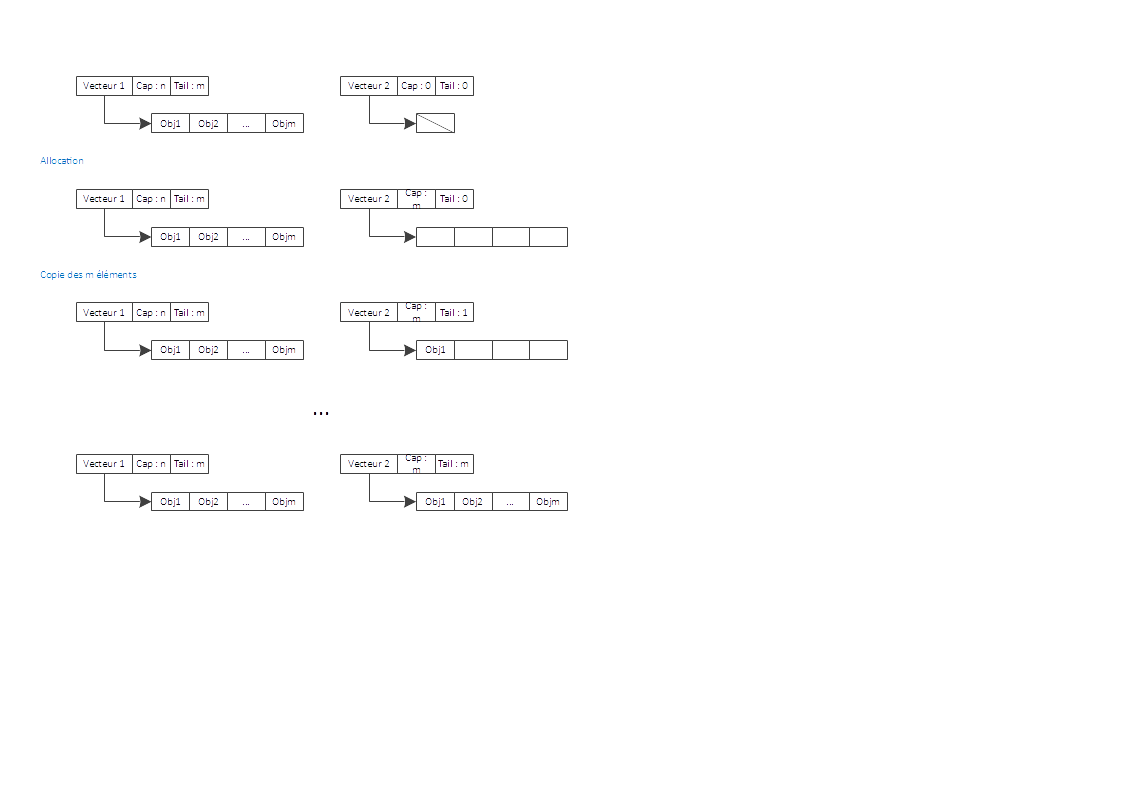
\includegraphics[height=0.7\textheight]{input_src/copie.png}
	\end{center}
\end{frame}

\begin{frame}
	\frametitle{Sémantique de déplacement\titlehfill{}3/7}
	\begin{itemize}
		\item Déplacement
	\end{itemize}

	\begin{center}
		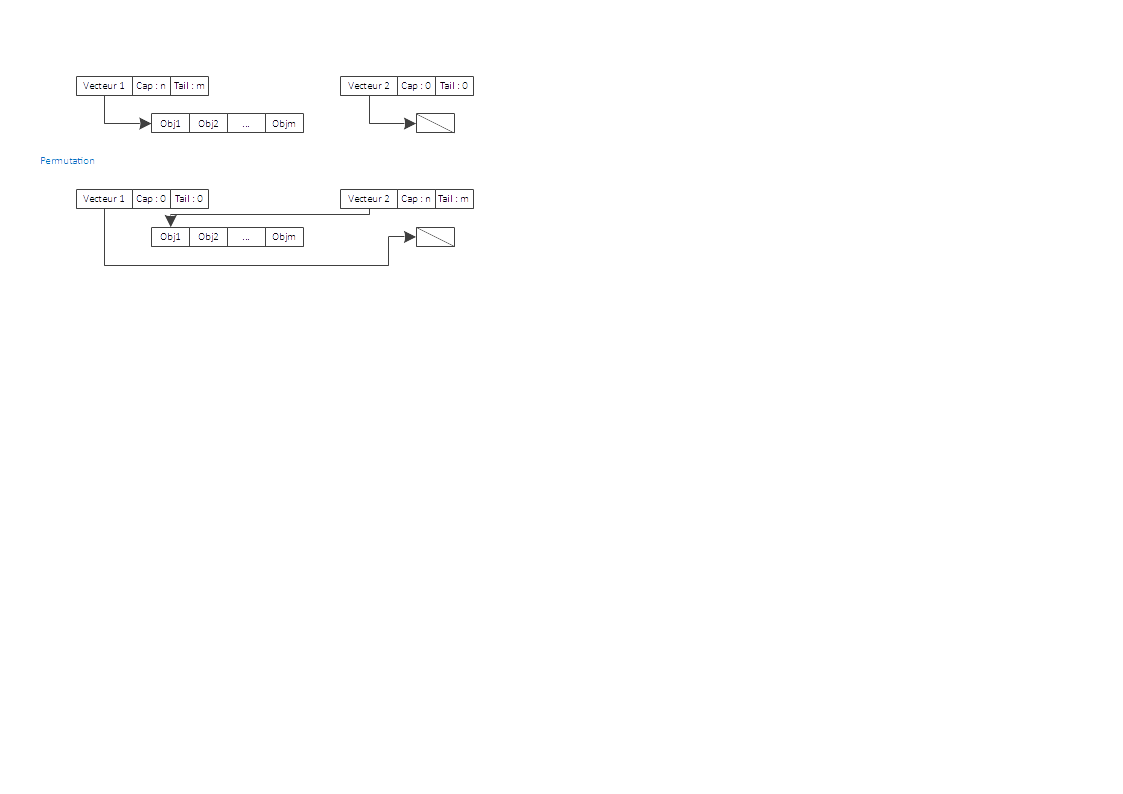
\includegraphics[height=0.4\textheight]{input_src/deplacement.png}
	\end{center}
\end{frame}

\begin{frame}[fragile]
	\frametitle{Sémantique de déplacement\titlehfill{}4/7}
	\begin{itemize}
		\item \textit{rvalue reference}
		\begin{itemize}
			\item Référence sur un objet temporaire ou sur le point d'être détruit
			\item Noté par une double esperluette : \lstinline|T&& value|
		\end{itemize}
		\item Deux fonctions \og de conversion\fg{}
		\begin{itemize}
			\item \lstinline|std::move()| convertit le paramètre en rvalue

\note[item]{\lstinline|std::move()| force la sémantique de déplacement sur l'objet}

			\item \lstinline|std::forward()| convertit le paramètre en \textit{rvalue} s'il n'est pas une \textit{lvalue reference}
		\end{itemize}

		\begin{block}{\textit{rvalue}, \textit{lvalue}, \ldots ?}
			Voir \href{http://www.open-std.org/jtc1/sc22/wg21/docs/papers/2012/n3337.pdf}{N3337} §3.10
		\end{block}

		\begin{block}{\lstinline|std::forward()| ?}
			Objectif : le \textit{perfect forwarding} (Voir \href{http://www.open-std.org/jtc1/sc22/wg21/docs/papers/2002/n1385.htm}{N1385})
		\end{block}
	\end{itemize}
\end{frame}

\begin{frame}
	\frametitle{Sémantique de déplacement\titlehfill{}5/7}
	\begin{itemize}
		\item Rendre une classe déplaçable
		\begin{itemize}
			\item Constructeur par déplacement \lstinline|T(const T&&)|
			\item Opérateur d'affectation par déplacement \lstinline|T& operator=(const T&&)|

			\begin{block}{Génération implicite}
				Pas de constructeur par copie, d'opérateur d'affectation, de destructeur, ni l'autre \og opérateur\fg{} de déplacement \textit{user-declared}
			\end{block}
		
			\begin{alertblock}{\textit{user-declared} ? \textit{user-provided} ?}
				\begin{itemize}
					\item \textit{user-declared} : la fonction est déclarée par l'utilisateur, y compris en \lstinline|= default| 
					\item \textit{user-provided} : le corps de la fonction est fourni par l'utilisateur

\note[item]{Pour faire simple un fonction \lstinline|=default| est \textit{user-declared} mais pas \textit{user-provided}. Dans le cas de la génération implicite des opérations de déplacement, c'est bien le \textit{user-declared} qui désactive.}
				\end{itemize}
			\end{alertblock}
		\end{itemize}
	\end{itemize}
\end{frame}

\begin{frame}
	\frametitle{Sémantique de déplacement\titlehfill{}6/7}
	\begin{block}{\textit{Rule of five}}
		Si une classe déclare destructeur, constructeur par copie, constructeur par déplacement, affectation par copie ou affectation par déplacement, alors elle doit définir les cinq

\note[item]{\textit{Rule of five} car constructeur par déplacement et opérateur d'affectation par déplacement ne sont pas générés implicitement si une autre des trois fonctions est déclarée par l'utilisateur}
\note[item]{Contrairement à \textit{Rule of three}, l'absence des constructeur et opérateur d'affectation par déplacement n'est pas une erreur grave, mais une optimisation manquée}
\note[item]{J'utilise déclare et non défini pour considérer \lstinline|=default| et \lstinline|=delete| qui peuvent être valables}
	\end{block}

	\begin{block}{\textit{Rule of zero}}
		Lorsque c'est possible, n'en définissez aucune

\note[item]{\textit{Rule of zero} s'applique typiquement aux classes sans gestion explicite d'\textit{ownership}, c'est à dire sans membres qu'il faut explicitement libérés, fermés, \ldots. Ce qui devrait être le cas par défaut.}
	\end{block}

	\begin{block}{Aller plus loin}
		Voir \href{https://github.com/cppp-france/CPPP-19/blob/master/elegance_style_epure_et_classe-Loic_Joly/elegance_style_epure_et_classe-Loic_Joly.pdf}{Élégance, style épuré et classe (Loïc Joly)}
	\end{block}
\end{frame}

\begin{frame}
	\frametitle{Sémantique de déplacement\titlehfill{}7/7}
	\begin{block}{Sémantique de déplacement dans la bibliothèque standard}
		\begin{itemize}
			\item Nombreuses classes standard déplaçables (thread, flux, \ldots)

\note[item]{Nombreuses classes déplaçables, y compris des classes non copiables}
\note[item]{Mutex et lock ne sont pas copiables ni déplaçables}

			\item Évolution de contraintes : déplaçable plutôt que copiable

\note[item]{Évolution des contraintes notamment pour les conteneurs et les algorithmes}
			
			\item Implémentations utilisent le déplacement si possible
		\end{itemize}
	\end{block}

	\begin{alertblock}{Bonnes pratiques ?}
		Nombreux débats sur les bonnes pratiques (existantes et nouvelles)

\note[item]{Débats sur les bonnes pratiques : nouvelles bonnes pratiques à définir et impact sur existant (\textit{rule of three}, élision de copie et RVO, forme canonique des opérateurs, surcharges)}
\note[item]{La situation a pu évoluer, je n'ai pas trop suivi le sujet}
	\end{alertblock}
\end{frame}

\subsection*{Initialisation}
\begin{frame}[fragile]
	\frametitle{Initializer list\titlehfill{}1/4}
	\begin{itemize}
		\item Initialisation des conteneurs
	\end{itemize}

	\begin{lstlisting}[language=C++]
vector<int> foo;

foo.push_back(1);
foo.push_back(56);
foo.push_back(18);
foo.push_back(3);

// Devient

vector<int> foo{1, 56, 18, 3};\end{lstlisting}
\end{frame}

\begin{frame}[fragile]
	\frametitle{Initializer list\titlehfill{}2/4}
	\begin{itemize}
		\item Une classe : \lstinline|std::initializer_list| pour accéder aux valeurs de la liste
	\end{itemize}

	\begin{alertblock}{Accéder, pas contenir !}
		\begin{itemize}
			\item \lstinline|std::initializer_list| référence mais ne contient pas les valeurs
			\item Contenues dans un tableau temporaire de même durée de vie
			\item Copier un \lstinline|std::initializer_list| ne copie pas les données
		\end{itemize}
	\end{alertblock}		

	\begin{itemize}
		\item Trois fonctions membres
		\begin{itemize}
			\item \lstinline|size()| : nombre d'éléments
			\item \lstinline|begin()| : itérateur de début de liste
			\item \lstinline|end()| : itérateur de fin de liste
		\end{itemize}
		\item Construction automatique depuis une liste de valeurs entre accolades
	\end{itemize}
\end{frame}

\begin{frame}[fragile]
	\frametitle{Initializer list\titlehfill{}3/4}
	\begin{itemize}
		\item Constructeurs peuvent prendre un \lstinline|std::initializer_list| en paramètre
	\end{itemize}

	\begin{lstlisting}[language=C++]
MaClasse(initializer_list<value_type> itemList);\end{lstlisting}

	\begin{itemize}
		\item \ldots ainsi que toute autre fonction
		\item Intégré aux conteneurs de la bibliothèque standard
	\end{itemize}
\end{frame}

\begin{frame}[fragile]
\frametitle{Initializer list\titlehfill{}4/4}
	\begin{exampleblock}{Do}
		Préférez \lstinline|std::initializer_list| aux insertions successives
	\end{exampleblock}

	\pause

	\begin{alertblock}{Don't}
		N'utilisez pas \lstinline|std::initializer_list| pour copier ou transformer, utilisez les algorithmes et constructeurs idoines

\note[item]{meilleure sémantique, plus évolutif et probablement plus performant}
	\end{alertblock}
\end{frame}

\begin{frame}[fragile]
	\frametitle{Uniform Initialization\titlehfill{}1/6}
	\begin{itemize}
		\item Plusieurs types d'initialisation en C++98/03 \ldots
	\end{itemize}

	\begin{lstlisting}[language=C++]
int a = 2;
int b(2);
int c[] = {1, 2, 3};
int d;\end{lstlisting}
\end{frame}

\begin{frame}[fragile]
	\frametitle{Uniform Initialization\titlehfill{}2/6}
	\begin{itemize}
		\item \ldots{}mais aucune de générique
	\end{itemize}

	\begin{lstlisting}[language=C++]
int a(2);        // Definition de l'entier a
int b();         // Declaration d'une fonction
int c(foo);      // ???
int d[] (1, 2);  // KO\end{lstlisting}

\note[item]{\lstinline|int b();| est un piège classique}
\note[item]{La signification de \lstinline|int c(foo);| va dépendre de ce qu'est \lstinline|foo|}

	\pause

	\begin{lstlisting}[language=C++]
int a[] = {1, 2, 3};        // OK

struct Foo { int a; };
Foo foo = {1};              // OK

vector<int> b = {1, 2, 3};  // KO
int c{8}                    // KO\end{lstlisting}

\note[item]{L'initialisation de \lstinline|Foo| fonctionne car c'est un POD (pas de classe de base, pas de virtuel, etc.)}
\end{frame}

\begin{frame}[fragile]
	\frametitle{Uniform Initialization\titlehfill{}3/6}
	\begin{itemize}
		\item En C++ 11, l'initialisation via \lstinline|{}| est générique
	\end{itemize}

	\begin{lstlisting}[language=C++]
int a[] = {1, 2, 3};         // OK
Foo b = {5};                 // OK
vector<int> c = {1, 2, 3};   // OK
int d = {8};                 // OK
int e = {};                  // OK\end{lstlisting}

	\pause

	\begin{itemize}
		\item Avec ou sans \lstinline|=|
	\end{itemize}

	\begin{lstlisting}[language=C++]
int a[]{1, 2, 3};            // OK
Foo b{5};                    // OK
vector<int> c{1, 2, 3};      // OK
int d{8};                    // OK
int e{};                     // OK\end{lstlisting}
\end{frame}

\begin{frame}[fragile]
	\frametitle{Uniform Initialization\titlehfill{}4/6}
	\begin{itemize}
		\item Dans différents contextes
	\end{itemize}

	\begin{lstlisting}[language=C++]
int* p = new int{4};
long l = long{2};

void f(int);
f({2});\end{lstlisting}
\end{frame}

\begin{frame}[fragile]
	\frametitle{Uniform Initialization\titlehfill{}5/6}
	\begin{alertblock}{Attention}
		Pas de troncature avec \lstinline|{}|

\note[item]{Ce qui, à mon avis, est plutôt une bonne chose}

		\begin{lstlisting}[language=C++]
int foo{2.5};  // Erreur\end{lstlisting}
	\end{alertblock}

	\pause

	\begin{alertblock}{Attention}
		Si le constructeur par \lstinline|std::initializer_list| existe, il est utilisé

		\begin{lstlisting}[language=C++]
vector<int> foo{2};  // 2
vector<int> foo(2);  // 0 0\end{lstlisting}
	\end{alertblock}
\end{frame}

\begin{frame}[fragile]
	\frametitle{Uniform Initialization\titlehfill{}6/6}
	\begin{alertblock}{Contraintes sur l'initialisation d'agrégats}
		\begin{itemize}
			\item Pas d'héritage
			\item Pas de constructeur fourni par l'utilisateur
			\item Pas d'initialisation \textit{brace-or-equal-initializers}
			\item Pas de fonction virtuelle ni de membre non statique protégé ou privé
		\end{itemize}

\note[item]{Initialisation par défaut sera abordée plus tard}
	\end{alertblock}

	\begin{exampleblock}{Do}
		Préférez l'initialisation \lstinline|{}| aux autres formes

\note[item]{Lorsque c'est possible, donc hors du cas du conteneur avec \textit{initiliazer list}}
	\end{exampleblock}

	\begin{exampleblock}{Do}
		Prenez garde à la différence entre \lstinline|std::vector<int> foo(2)| et \lstinline|std::vector<int> foo{2}|
	\end{exampleblock}
\end{frame}

\subsection*{Déduction de type}
\begin{frame}[fragile]
	\frametitle{\lstinline|auto|\titlehfill{}1/6}
	\begin{itemize}
		\item Déduction (inférence) de type

\note[item]{Les deux termes se trouvent. Notammment car c'est une forme simple (par rapport à des langages fonctionnels comme Caml ou Haskell) de l'inférence.}

		\item Type se déduit de l'initialisation
	\end{itemize}

	\pause

	\begin{alertblock}{Inférence de type $\neq$ typage dynamique}
		Deux notions orthogonales, le typage reste statique
	\end{alertblock}

	\begin{alertblock}{Inférence de type $\neq$ typage faible}
		Encore deux notions orthogonales
	\end{alertblock}

	\begin{alertblock}{typage dynamique $\neq$ typage faible}
		Toujours deux notions orthogonales

\note[item]{Contre-exemple le C est statiquement typé mais pas très fortement (conversions implicites) et moins que ne l'est le Python pourtant dynamiquement typé}
\note[item]{Pour le C++, la remarque est partiellement vraie, mais il élimine malgré tout certains typages implicites, offre beaucoup plus d'outils pour un bon typage et surtout encourage un typage fort. La faiblesse résiduelle est une conséquence de l'héritage du C et de la forte compatibilité avec celui-ci et n'est en pratique utilisée que dans la partie \og bas niveau\fg{} du C++}
	\end{alertblock}
\end{frame}

\begin{frame}[fragile]
	\frametitle{\lstinline|auto|\titlehfill{}2/6}
	\begin{block}{Typage \& vocabulaire}
		\begin{itemize}
			\item Statique : type porté par la variable et ne varie pas
			\item Dynamique : type porté par la valeur, le type de la variable change au fil des affectations
			\item Absence : variable non typée, le type est imposé par l'opération
			\item Parfois une distinction \textit{compile-time} / \textit{run-time}

\note[item]{La distinction \textit{run-time} / \textit{compile-time} est globalement compatible, au moins à première vue, avec l'explication au dessus mais est à mon sens trop ad-hoc et surtout laisse imaginer que typage dynamique = interprété et typage statique = compilé et que l'on ne peut faire aucune vérifications statique de types en typage dynamique ce qui n'est pas totalement vrai (voir linter)}
		\end{itemize}
	\end{block}
\end{frame}

\begin{frame}[fragile]
	\frametitle{\lstinline|auto|\titlehfill{}3/6}
	\begin{itemize}
		\item \lstinline|auto| définit une variable dont le type est déduit
	\end{itemize}

	\begin{lstlisting}[language=C++]
auto i = 2;  // int\end{lstlisting}

	\begin{itemize}
		\item Règles de déduction proches de celles des \textit{templates}
		\item Listes entre accolades inférées comme des \lstinline|std::initializer_list|
	\end{itemize}

	\begin{alertblock}{Attention}
		Référence, \lstinline|const| et \lstinline|volatile| sont perdus durant la déduction

		\begin{lstlisting}[language=C++]
const int i = 2;
auto j = i;  // int \end{lstlisting}
	\end{alertblock}
\end{frame}

\begin{frame}[fragile]
	\frametitle{\lstinline|auto|\titlehfill{}4/6}
	\begin{itemize}
		\item Combinaison possible avec \lstinline|const|, \lstinline|volatile| ou \lstinline|&|
	\end{itemize}

	\begin{lstlisting}[language=C++]
const auto i = 2;

int j = 3;
auto& k = j;\end{lstlisting}

	\begin{itemize}
		\item Typer explicitement l'initialiseur permet de forcer le type déduit
	\end{itemize}

	\begin{lstlisting}[language=C++]
// unsigned long
auto i = static_cast<unsigned long>(2);
auto j = 2UL\end{lstlisting}
\end{frame}

\begin{frame}[fragile]
	\frametitle{\lstinline|auto|\titlehfill{}5/6}
	\begin{itemize}
		\item Une tendance forte : \textit{Almost Always Auto} (AAA)

		\begin{block}{Pour aller plus loin}
			Voir \href{https://herbsutter.com/2013/08/12/gotw-94-solution-aaa-style-almost-always-auto/}{GotW 94 : AAA Style}
		\end{block}

		\item Plusieurs avantages (robustesse, performances, maintenabilité, \ldots)
		\begin{itemize}
			\item Variables forcément initialisées
			\item Typage correct et précis
			\item Garanties conservées au fil des corrections et refactoring
			\item Généricité et simplification du code

\note[item]{Simplification du code, voir exemple des itérateurs}
\note[item]{Également une forte résistance, mais davantage de la part \og d'anonyme\fg{}}
		\end{itemize}
	\end{itemize}

	\onslide<2-3>
	\begin{block}{Quiz}
		Quelle est le type de retour de la fonction membre \lstinline|size()| d'une \lstinline|std::list<std::string>| ?
	\end{block}

	\onslide<3>
	\begin{block}{Réponse}
		\lstinline|std::list<std::string>::size_type|
	\end{block}
\end{frame}

\begin{frame}[fragile]
	\frametitle{\lstinline|auto|\titlehfill{}6/6}
	\begin{itemize}
		\item Limitations - solutions
		\begin{itemize}
			\item Erreur de déduction de type - typage explicite de l'initialiseur
			\item Pas d'initialisation possible - \lstinline|decltype|
			\item Interfaces, rôles, contexte - concepts ?

\note[item]{Pas utile de connaitre le type exact d'une variables de type \lstinline|std::map<std::string, std::vector<unsigned long long> >::const_iterator| mais il peut être important de savoir que c'est un itérateur. Ce qu'auto n'indique pas}
\note[item]{Mais il faut attendre C++20 pour avoir les concepts}
		\end{itemize}
	\end{itemize}

	\begin{block}{Mon point de vue sur AAA}
		\begin{itemize}
			\item Arguments en faveur de AAA convaincants
			\item Mais les vieilles habitudes sont dures à perdre
		\end{itemize}
	\end{block}

	\begin{alertblock}{Compatibilité}
		Mot clé \lstinline|auto| présent en C++98/03 avec un sens radicalement différent

\note[item]{Sens en C++98/03 : variable de type automatique (c'est à dire sur la pile) par opposition à statique. Inutile car c'est le cas par défaut et donc inutilisé}
\note[item]{Un cas où la compatibilité ascendante entre C++98/03 et C++11 a été rompue}
	\end{alertblock}

	\begin{block}{Dépréciation}
		Mot-clé \lstinline|register| également déprécié

\note[item]{\lstinline|register| est supprimé en C++17}
	\end{block}
\end{frame}

\begin{frame}[fragile]
	\frametitle{\lstinline|decltype|}
	\begin{itemize}
		\item \lstinline|decltype| déduit le type d'une variable ou d'une expression
		\item Et permet donc de créer une variable du même type
	\end{itemize}

	\begin{lstlisting}[language=C++]
int a;
long b;
decltype(a) c;     // int
decltype(a + b) d; // long\end{lstlisting}

	\begin{itemize}
		\item Généralement, déduction sans aucune modification du type

\note[item]{Donc conservation des référénces, const, etc.}

		\item Depuis une \textit{lvalue} de type \lstinline|T| autre qu'un nom de variable : \lstinline|T&|
	\end{itemize}

	\begin{lstlisting}[language=C++]
decltype( (a) ) e;     // int&\end{lstlisting}

\note[item]{Au passage, cette ligne ne compile pas car la référence n'est pas initialisée}
\end{frame}

\begin{frame}[fragile]
	\frametitle{\lstinline|declval|}
	\begin{itemize}
		\item Permet l'utilisation de fonctions membres dans \lstinline|decltype| sans appel au constructeur
		\item Typiquement sur des templates acceptant des types sans constructeur commun mais avec une fonction membre commune
	\end{itemize}
	
	\begin{lstlisting}[language=C++]
struct foo {
  foo(const foo&) { }
  int bar () const { return 1; } };

decltype(foo().bar()) n2 = 5;               // Erreur
decltype(std::declval<foo>().bar()) n2 = 5; // OK, int\end{lstlisting}

	\begin{alertblock}{Attention}
		Uniquement dans des contextes non évalués
	\end{alertblock}
\end{frame}

\begin{frame}[fragile]
	\frametitle{Déduction du type retour\titlehfill{}1/2}
	\begin{itemize}
		\item \lstinline|auto| et \lstinline|decltype| permettent de déduire le type retour d'une fonction
	\end{itemize}

	\begin{lstlisting}[language=C++]
auto add(int a, int b) -> decltype(a + b) {
  return a + b; }\end{lstlisting}

	\begin{itemize}
		\item Particulièrement utiles pour des fonctions template
	\end{itemize}

	\onslide<2>
	\begin{block}{Quiz : Que mettre à la place des XXX ? T, U, autre chose ?}
		\begin{lstlisting}[language=C++]
template<typename T, typename U> XXX add(T a, U b) {
  return a + b; }\end{lstlisting}

\note[item]{Vrai problème sur les templates avant C++11}
\note[item]{Une solution historique : un seul type template et on compte sur les conversions implicites voire on demande des conversions explicites}
	\end{block}
\end{frame}

\begin{frame}[fragile]
	\frametitle{Déduction du type retour\titlehfill{}2/2}
	\begin{block}{Solution}
		\begin{itemize}
			\item Pas de bonnes réponses en typage explicite
			\item Mais l'inférence de type vient à notre secours
		\end{itemize}
	\end{block}

	\begin{lstlisting}[language=C++]
template<typename T, typename U>
auto add(T a, U b) -> decltype(a + b) {
  return a + b; }\end{lstlisting}

	\begin{exampleblock}{do}
		Utilisez la déduction du type retour dans vos fonctions templates
	\end{exampleblock}
\end{frame}

\subsection*{Conteneurs}
\begin{frame}[fragile]
	\frametitle{Conteneurs\titlehfill{}1/5}
	\begin{itemize}
		\item \lstinline|std::array|
		\begin{itemize}
			\item tableau de taille fixe connue à la compilation
			\item Éléments contigus
			\item Accès indexé
		\end{itemize}
	\end{itemize}

	\begin{lstlisting}[language=C++]
array<int, 8> foo{2, 5, 9, 8, 2, 6, 8, 9};
accumulate(foo.begin(), foo.end(), 0); // 49\end{lstlisting}

	\begin{lstlisting}[language=C++]
array<int, 8> foo{2, 5, 9, 8, 2, 6, 8, 9, 17};
// Erreur de compilation\end{lstlisting}

\begin{itemize}
	\item[]\begin{itemize}
		\item Permet la vérification des index à la compilation
	\end{itemize}
\end{itemize}

\note[item]{Des implémentations peuvent aussi proposer une assertion sur \lstinline|operator[]| permettant une détection des erreurs à l'exécution en debug (p.ex. sur les TU)}

		\begin{lstlisting}[language=C++]
array<int, 8> foo{2, 5, 9, 8, 2, 6, 8, 9};
cout << get<2>(foo) << '\n';  // 9
cout << get<8>(foo) << '\n';  // Erreur de compilation\end{lstlisting}
\end{frame}

\begin{frame}[fragile]
\frametitle{Conteneurs\titlehfill{}2/6}
	\begin{itemize}
		\item \lstinline|std::forward_list| : liste simplement chaînée
	\end{itemize}

	\begin{lstlisting}[language=C++]
forward_list<int> foo{2, 5, 9, 8, 2, 6, 8, 9, 12};
accumulate(foo.begin(), foo.end(), 0); // 61\end{lstlisting}
\end{frame}

\begin{frame}[fragile]
	\frametitle{Conteneurs\titlehfill{}3/6}
	\begin{itemize}
		\item Conteneurs associatifs sous forme de tables de hachage
		\begin{itemize}
			\item \lstinline|std::unordered_map|
			\item \lstinline|std::unordered_multimap|
			\item \lstinline|std::unordered_set|
			\item \lstinline|std::unordered_multiset|
		\end{itemize}
		\item Versions non ordonnées de \lstinline|std::map|, \lstinline|std::multimap|, \lstinline|std::set| et \lstinline|std::multiset|

		\begin{block}{Pourquoi unordered ?}
			\begin{itemize}
				\item Trop nombreuses implémentations \lstinline|hash_XXX| existantes
				\item Structures fondamentalement non ordonnées
			\end{itemize}
		\end{block}
	\end{itemize}
\end{frame}

\begin{frame}[fragile]
	\frametitle{Conteneurs\titlehfill{}4/6}
	\begin{itemize}
		\item \lstinline|shrink_to_fit()| réduit la capacité des \lstinline|std::vector|, \lstinline|std::deque| et \lstinline|std::string| à leur taille
	\end{itemize}

\note[item]{Pour être précis, ce n'est pas nécessairement exactement à la taille ça peut être plus grand - à la discrétion de l'implémentation (performances, cohérence, \ldots) -, mais l'idée est là}

	\begin{lstlisting}[language=C++]
vector<int> foo{12, 25};
foo.reserve(15);
// Taille : 2, capacite : 15

foo.shrink_to_fit();
// Taille : 2, capacite : 2\end{lstlisting}

	\begin{itemize}
		\item \lstinline|data()| récupère le \og tableau C\fg{} d'un \lstinline|std::vector|
	\end{itemize}

	\begin{block}{\lstinline|foo.data()| ou \lstinline|&foo[0]|}
		\begin{itemize}
			\item Comportement identique
			\item Préférez \lstinline|foo.data()| sémantiquement plus clair
		\end{itemize}
	\end{block}
\end{frame}

\begin{frame}[fragile]
	\frametitle{Conteneurs\titlehfill{}5/6}
	\begin{itemize}
		\item \lstinline|emplace()|, \lstinline|emplace_back()| et \lstinline|emplace_front()| construisent directement dans le conteneur depuis les paramètres d'un des constructeurs de l'élément
	\end{itemize}

	\begin{lstlisting}[language=C++]
class Point {
public:
  Point(int a, int b); };

vector<Point> foo;
foo.emplace_back(2, 5);\end{lstlisting}

	\begin{block}{Objectif}
		Éliminer les copies inutiles restantes et gagner en performance

\note[item]{Copies  présentes malgré l'élision de copie, (N)RVO et la sémantique de déplacement}
\note[item]{On gagne aussi en lisibilité (moins de ligne, pas de construction juste pour pousser, pas d'introduction d'un nom sans utilité)}
	\end{block}
\end{frame}

\begin{frame}[fragile]
	\frametitle{Conteneurs\titlehfill{}6/6}
	\begin{itemize}
		\item Évolutions de \lstinline|std::string|
		\begin{itemize}
			\item Éléments obligatoirement contigus
			\item \lstinline|data()| retourne une chaîne C valide (synonyme à \lstinline|c_str()|)

\note[item]{En C++98, \lstinline|data()| renvoyait les caractères de la chaîne mais pas nécessairement sous forme d'une chaîne C valide (pas obligatoirement de 0 terminal)}

			\item \lstinline|front()| retourne le premier caractère d'une chaîne
			\item \lstinline|back()| retourne le dernier caractère d'une chaîne
			\item \lstinline|pop_back()| supprime le dernier caractère d'une chaîne
		\end{itemize}
		\item Évolutions de \lstinline|std::bitset|
		\begin{itemize}
			\item \lstinline|all()| teste si tous les bits sont levés
			\item \lstinline|to_ullong()| converti en \lstinline|unsigned long long|
		\end{itemize}
	\end{itemize}

	\begin{exampleblock}{Do}
		\begin{itemize}
			\item Préférez \lstinline|std::array| lorsque la taille est fixe et connue
			\item Sinon préférez \lstinline|std::vector| 
		\end{itemize}
	\end{exampleblock}
\end{frame}

\subsection*{Itérateurs}
\begin{frame}[fragile]
	\frametitle{Itérateurs\titlehfill{}1/4}
	\begin{itemize}
		\item Fonctions membres \lstinline|cbegin()|, \lstinline|cend()|, \lstinline|crbegin()| et \lstinline|rcend()| permettant d'obtenir systématiquement des \lstinline|const_iterator|

\note[item]{Les fonctions \lstinline|begin()|, \lstinline|end()|, etc. retournent des \lstinline|const_iterator| si le conteneur est const, des iterator dans le cas contraire}

		\item Fonctions libres \lstinline|std::begin()| et \lstinline|std::end()|
		\begin{itemize}
			\item conteneur : équivalente aux fonctions membres
			\item tableau C : adresse du premier élément et suivant le dernier élément
		\end{itemize}
	\end{itemize}

	\begin{lstlisting}[language=C++]
int foo[] = {1, 2, 3, 4};
vector<int> bar{2, 3, 4, 5};

accumulate(begin(foo), end(foo), 0);  // 10
accumulate(begin(bar), end(bar), 0);  // 14\end{lstlisting}
\end{frame}

\begin{frame}[fragile]
	\frametitle{Itérateurs\titlehfill{}2/4}
	\begin{itemize}
		\item Fonctions libres \lstinline|std::begin()| et \lstinline|std::end()| (cont.)
		\begin{itemize}
			\item compatibles avec les conteneurs non-STL proposant les fonctions membres \lstinline|begin()| et \lstinline|end()|
			\item Surchargeable sans modification du conteneur pour les autres

\note[item]{Surcharge : respect de OCP.}
		\end{itemize}
	\end{itemize}

	\begin{lstlisting}[language=C++]
class Foo {
public:
  char* first();
  const char* first() const; };

char* begin(Foo& foo) {
  return foo.first();}

const char* begin(const Foo& foo) {
  return foo.first();}\end{lstlisting}
\end{frame}

\begin{frame}[fragile]
	\frametitle{Itérateurs\titlehfill{}3/4}
	\begin{block}{Conseils}
		\lstinline|using std::begin| et \lstinline|using std::end| pour permettre à l'ADL de fonctionner malgré la surcharge
	\end{block}

	\begin{alertblock}{Don't}
		N'ouvrez pas le namespace \lstinline|std| pour spécialiser
	\end{alertblock}

	\begin{exampleblock}{Do}
		Préférez \lstinline|std::begin()| et \lstinline|std::end()| aux fonctions membres

\note[item]{Plus générique (à commencer par tableau C), coût à priori nul}
	\end{exampleblock}
\end{frame}

\begin{frame}[fragile]
	\frametitle{Itérateurs\titlehfill{}4/4}
	\begin{itemize}
		\item Fonctions libres \lstinline|std::prev()| et \lstinline|std::next()| permettant de retrouver l'itérateur suivant ou précédant un itérateur
		\item \lstinline|move_iterator| : adaptateur d'itérateur retournant des \textit{rvalue reference} lors du déréférencement
	\end{itemize}

	\begin{lstlisting}[language=C++]
vector<string> foo(3), bar{"one","two","three"};

typedef vector<string>::iterator Iter;

copy(move_iterator<Iter>(bar.begin()),
     move_iterator<Iter>(bar.end()),
     foo.begin());
// foo : "one" "two" "three"
// bar : "" "" ""\end{lstlisting}

\note[item]{Exemple repris de www.cpluplus.com.}
\end{frame}

\subsection*{Algorithmes}
\begin{frame}[fragile]
	\frametitle{Foncteurs prédéfinis}
	\begin{itemize}
		\item \lstinline|std::bit_and()| : et bit à bit
		\item \lstinline|std::bit_or()| : ou inclusif bit à bit
		\item \lstinline|std::bit_xor()| : ou exclusif bit à bit
	\end{itemize}

	\begin{lstlisting}[language=C++]
vector<unsigned char> foo{0x10, 0x20, 0x30};
vector<unsigned char> bar{0xFF, 0x25, 0x00};
vector<unsigned char> baz;

transform(begin(foo), end(foo), begin(bar), 
back_inserter(baz), 
bit_and<unsigned char>());
// baz : 0x10 0x20, 0x00\end{lstlisting}
\end{frame}

\begin{frame}[fragile]
	\frametitle{Algorithmes - Recherche linéaire}
	\begin{itemize}
		\item \lstinline|std::find_if_not()| recherche le premier élément ne vérifiant pas le prédicat
	\end{itemize}

	\begin{lstlisting}[language=C++]
vector<int> foo{1, 4, 5, 9, 12};

find_if_not(begin(foo), end(foo), isOdd); // 4\end{lstlisting}

\note[item]{Similaire à \lstinline|std::find_if| avec le prédicat nié, mais sémantiquement plus clair}
\end{frame}

\begin{frame}[fragile]
	\frametitle{Algorithmes - Comparaison\titlehfill{}1/4}
	\begin{itemize}
		\item \lstinline|std::all_of()| indique si tous les éléments de l'ensemble vérifient un prédicat
	\end{itemize}

	\begin{lstlisting}[language=C++]
vector<int> foo{1, 4, 5, 9, 12};
vector<int> bar{1, 5, 9};
vector<int> baz{4, 12};

all_of(begin(foo), end(foo), isOdd); // False
all_of(begin(bar), end(bar), isOdd); // True
all_of(begin(baz), end(baz), isOdd); // False\end{lstlisting}

	\begin{itemize}
		\item Retourne vrai si l'ensemble est vide
	\end{itemize}
\end{frame}

\begin{frame}[fragile]
	\frametitle{Algorithmes - Comparaison\titlehfill{}2/4}
	\begin{itemize}
		\item \lstinline|std::any_of()| indique si au moins un élément de l'ensemble vérifie un prédicat
	\end{itemize}

	\begin{lstlisting}[language=C++]
vector<int> foo{1, 4, 5, 9, 12};
vector<int> bar{1, 5, 9};
vector<int> baz{4, 12};

any_of(begin(foo), end(foo), isOdd); // True
any_of(begin(bar), end(bar), isOdd); // True
any_of(begin(baz), end(baz), isOdd); // False\end{lstlisting}

	\begin{itemize}
		\item Retourne faux si l'ensemble est vide
	\end{itemize}
\end{frame}

\begin{frame}[fragile]
	\frametitle{Algorithmes - Comparaison\titlehfill{}3/4}
	\begin{itemize}
		\item \lstinline|std::none_of()| indique si aucun élément de l'ensemble ne vérifie le prédicat
	\end{itemize}

	\begin{lstlisting}[language=C++]
vector<int> foo{1, 4, 5, 9, 12};
vector<int> bar{1, 5, 9};
vector<int> baz{4, 12};

none_of(begin(foo), end(foo), isOdd); // False
none_of(begin(bar), end(bar), isOdd); // False
none_of(begin(baz), end(baz), isOdd); // True\end{lstlisting}

	\begin{itemize}
		\item Retourne vrai si l'ensemble est vide
	\end{itemize}
\end{frame}

\begin{frame}[fragile]
	\frametitle{Algorithmes - Comparaison\titlehfill{}4/4}
	\begin{itemize}
		\item \lstinline|std::is_permutation()| indique si un ensemble est la permutation d'un autre
	\end{itemize}

	\begin{lstlisting}[language=C++]
vector<int> foo{1, 4, 5, 9, 12};
vector<int> bar{1, 5, 4, 9, 12};
vector<int> baz{5, 4, 3, 9, 1};

is_permutation(begin(foo), end(foo), begin(bar)); // true
is_permutation(begin(foo), end(foo), begin(baz)); // false\end{lstlisting}

	\begin{itemize}
		\item Égalité des éléments mais pas de leur ordre
	\end{itemize}
\end{frame}

\begin{frame}[fragile]
	\frametitle{Algorithmes - Copie}
	\begin{itemize}
		\item \lstinline|std::copy_n()| copie les n premiers éléments d'un ensemble
	\end{itemize}

	\begin{lstlisting}[language=C++]
vector<int> foo{1, 4, 5, 9, 12}, bar;

copy_n(begin(foo), 3, back_inserter(bar)); // 1 4 5\end{lstlisting}

	\begin{itemize}
		\item \lstinline|std::copy_if()| copie les éléments vérifiant un prédicat
	\end{itemize}

	\begin{lstlisting}[language=C++]
vector<int> foo{1, 4, 5, 9, 12}, bar;

copy_if(begin(foo), end(foo), back_inserter(bar), isOdd);
// 1 5 9\end{lstlisting}
\end{frame}

\begin{frame}[fragile]
	\frametitle{Algorithmes - Déplacement}
	\begin{itemize}
		\item \lstinline|std::move()| déplace les éléments d'un ensemble (du début vers la fin)
	\end{itemize}

	\begin{lstlisting}[language=C++]
vector<int> foo{4, 5, 9, 12};
vector<int> bar;

move(begin(foo), end(foo), back_inserter(bar));\end{lstlisting}

	\begin{itemize}
		\item \lstinline|std::move_backward()| déplace les éléments (de la fin vers le début)
		\item Versions \og déplacement\fg{} de \lstinline|std::copy()| et \lstinline|std::copy_backward()|
	\end{itemize}
\end{frame}

\begin{frame}[fragile]
	\frametitle{Algorithmes - Partitionnement\titlehfill{}1/2}
	\begin{itemize}
		\item \lstinline|std::is_partitioned()| indique si un ensemble est partitionné, c'est à dire si les éléments vérifiant un prédicat sont avant ceux ne le vérifiant pas
	\end{itemize}

	\begin{lstlisting}[language=C++]
vector<int> foo{4, 5, 9, 12};
vector<int> bar{9, 5, 4, 12};

is_partitioned(begin(foo), end(foo), isOdd); // false
is_partitioned(begin(bar), end(bar), isOdd); // true\end{lstlisting}
\end{frame}

\begin{frame}[fragile]
	\frametitle{Algorithmes - Partitionnement\titlehfill{}2/2}
	\begin{itemize}
		\item \lstinline|std::partition_copy()| copie l'ensemble en le partitionnant
		\item \lstinline|std::partition_point()| retourne le point de partition d'un ensemble partitionné, c'est à dire le premier élément ne vérifiant pas le prédicat
	\end{itemize}

	\begin{lstlisting}[language=C++]
vector<int> foo{9, 5, 4, 12};

partition_point(begin(foo), end(foo), isOdd); // 4\end{lstlisting}
\end{frame}

\begin{frame}[fragile]
	\frametitle{Algorithmes - Tri}
	\begin{itemize}
		\item \lstinline|std::is_sorted()| indique si l'ensemble est ordonnée (ascendant)
	\end{itemize}

\note[item]{Possibilité de fournir un foncteur de comparaison (\lstinline|<| par défaut)}

	\begin{lstlisting}[language=C++]
vector<int> foo{4, 5, 9, 12};
vector<int> bar{9, 5, 4, 12};

is_sorted(begin(foo), end(foo)); // true
is_sorted(begin(bar), end(bar)); // false\end{lstlisting}

	\begin{itemize}
		\item \lstinline|std::is_sorted_until()| détermine le premier élément non ordonné
	\end{itemize}

	\begin{lstlisting}[language=C++]
vector<int> foo{4, 5, 9, 3, 12};

is_sorted_until(begin(foo), end(foo)); // 3\end{lstlisting}
\end{frame}

\begin{frame}[fragile]
	\frametitle{Algorithmes - Mélange}
	\begin{itemize}
		\item \lstinline|std::shuffle()| mélange l'ensemble grâce à un générateur de nombre aléatoire \og uniforme\fg{}
	\end{itemize}

	\begin{lstlisting}[language=C++]
vector<int> foo{4, 5, 9, 12};
unsigned seed = now().time_since_epoch().count();

shuffle(begin(foo), end(foo), default_random_engine(seed));\end{lstlisting}

\note[item]{Générateurs de nombre aléatoire correspondant vus plus tard}
\end{frame}

\begin{frame}[fragile]
	\frametitle{Algorithmes - Gestion de \og tas\fg{}}
	\begin{itemize}
		\item \lstinline|std::is_heap()| indique si l'ensemble forme un tas
	\end{itemize}

	\begin{lstlisting}[language=C++]
vector<int> foo{4, 5, 9, 3, 12};

is_heap(begin(foo), end(foo));  // false
make_heap(begin(foo), end(foo));
is_heap(begin(foo), end(foo));  // true\end{lstlisting}

	\begin{itemize}
		\item \lstinline|std::is_heap_until()| indique le premier élément qui n'est pas dans la position correspondant à un tas 
	\end{itemize}
\end{frame}

\begin{frame}[fragile]
	\frametitle{Algorithmes - Min-max}
	\begin{itemize}
		\item \lstinline|std::minmax()| retourne la paire constituée du plus petit et du plus grand de deux éléments
	\end{itemize}

	\begin{lstlisting}[language=C++]
minmax(5, 2); // 2 - 5\end{lstlisting}

	\begin{itemize}
		\item \lstinline|std::minmax_element()| retourne la paire constituée des itérateurs sur le plus petit et le plus grand élément d'un ensemble
	\end{itemize}

	\begin{lstlisting}[language=C++]
vector<int> foo{18, 5, 6, 8};

minmax_element(foo.begin(), foo.end()); // 5 - 18\end{lstlisting}

\note[item]{La fonction de comparaison est configurable (< par défaut)}
\note[item]{Globalement une combinaison des fonctions min et max en un seul parcours}
\note[item]{Optimisation hyper classique de rechercher min et max en un seul parcours}
\end{frame}

\begin{frame}[fragile]
	\frametitle{Algorithmes - Numérique}
	\begin{itemize}
		\item \lstinline|std::iota()| affecte des valeurs successives aux éléments d'un ensemble
	\end{itemize}

	\begin{lstlisting}[language=C++]
vector<int> foo(5);

iota(begin(foo), end(foo), 50); // 50 51 52 53 54\end{lstlisting}
\end{frame}

\begin{frame}[fragile]
	\frametitle{Algorithmes - Conclusion}
	\begin{exampleblock}{Do}
		Continuez à suivre les règles C++98/03 à propos des algorithmes
	\end{exampleblock}

	\begin{exampleblock}{Do}
		Privilégiez la sémantique lorsque plusieurs algorithmes sont utilisables
	\end{exampleblock}
\end{frame}

\subsection*{range-based for loop}
\begin{frame}[fragile]
	\frametitle{\textit{Range-based for loop}\titlehfill{}1/3}
	\begin{itemize}
		\item Itération sur un \og conteneur\fg{} complet
	\end{itemize}

	\begin{lstlisting}
vector<int> foo{4, 8, 12, 37};
for(int var : foo)
  cout << var << " ";    // Affiche 4 8 12 37\end{lstlisting}

	\begin{itemize}
		\item Compatible avec \lstinline|auto|
	\end{itemize}

	\begin{lstlisting}
vector<int> foo{4, 8, 12, 37};
for(auto var : foo)
  cout << var << " ";    // Idem\end{lstlisting}
\end{frame}

\begin{frame}[fragile]
	\frametitle{\textit{Range-based for loop}\titlehfill{}2/3}
	\begin{alertblock}{Modification}
		Pour modifier les éléments du conteneur la variable d'itération doit être une référence
	\end{alertblock}

	\begin{lstlisting}
vector<int> foo(4);

for(auto& var : foo)
  var = 5;    // foo : 5 5 5 5\end{lstlisting}

	\begin{itemize}
		\item Utilisable sur tout conteneur
		\begin{itemize}
			\item Exposant \lstinline|begin()| et \lstinline|end()| ou
			\item Utilisable avec \lstinline|std::begin()| et \lstinline|std::end()|
		\end{itemize}
	\end{itemize}
\end{frame}

\begin{frame}
	\frametitle{\textit{Range-based for loop}\titlehfill{}3/3}
	\begin{exampleblock}{Do}
		Préférez \textit{range-based for loop} aux boucles for classiques et à l'algorithme \lstinline|std::for_each()|
	\end{exampleblock}

	\begin{block}{Conseils}
		\begin{itemize}
			\item Contrairement à for(;;), l'indice de l'itération n'est pas disponible
			\item Malgré tout, préférez la \textit{range-based for loop} avec un indice externe au for classique
			\item Plus robuste, plus sûr

\note[item]{Motivation : gestion d'indice en plusieurs endroits plus complexe à lire et source d'erreur sur celui-ci (incrémentation) mais garantie de ne pas dépasser les bornes ce qui est une erreur bien moins évidente à détecter en test et plus dangeureuse}
		\end{itemize}
	\end{block}

	\begin{exampleblock}{Do}
		Utilisez l'inférence de type sur la variable d'itération
	\end{exampleblock}
\end{frame}

\subsection*{string et conversions}
\begin{frame}[fragile]
	\frametitle{\lstinline|std::string| \& conversions\titlehfill{}1/3}
	\begin{itemize}
		\item Fonctions de conversion d'une chaîne de caractères en un nombre
		\begin{itemize}
			\item \lstinline|std::stoi()| vers int
			\item \lstinline|std::stol()| vers long
			\item \lstinline|std::stoul()| vers unsigned long
			\item \lstinline|std::stoll()| vers long long
			\item \lstinline|std::stoull()| vers unsigned long long
			\item \lstinline|std::stof()| vers float
			\item \lstinline|std::stod()| vers double
			\item \lstinline|std::stold()| vers long double
		\end{itemize}
	\end{itemize}

	\begin{lstlisting}
cout << stoi("56"); // Affiche 56\end{lstlisting}

	\begin{itemize}
		\item S'arrêtent sur le premier caractère non convertible
	\end{itemize}
\end{frame}

\begin{frame}[fragile]
	\frametitle{\lstinline|std::string| \& conversions\titlehfill{}2/3}
	\begin{itemize}
		\item \lstinline|std::to_string()| : conversion d'un nombre en une chaîne de caractères
	\end{itemize}

	\begin{lstlisting}
cout << to_string(56); // Affiche 56\end{lstlisting}

	\begin{itemize}
		\item \lstinline|std::to_wstring()| : conversion vers une chaîne de caractères larges
	\end{itemize}
\end{frame}

\begin{frame}[fragile]
	\frametitle{\lstinline|std::string| \& conversions\titlehfill{}3/3}
	\begin{alertblock}{Attention}
		Pas de fonction \lstinline|std::stoui()| de conversion vers un unsigned int
	\end{alertblock}

	\begin{exampleblock}{Do}
		Préférez \lstinline|std::sto<X>()| à \lstinline|sscanf()|, \lstinline|atoi()| ou \lstinline|strto<X>()|
	\end{exampleblock}

	\begin{exampleblock}{Do}
		Préférez \lstinline|std::to_string()| à \lstinline|s(n)printf()| ou \lstinline|itoa()|
	\end{exampleblock}

	\begin{block}{Alternative et complément}
		Boost.Lexical\_cast permet également de telles conversions et quelques autres
	\end{block}
\end{frame}

\subsection*{string UTF}
\begin{frame}[fragile]
	\frametitle{Chaînes de caractères UTF}
	\begin{itemize}
		\item \lstinline|char| doit pouvoir contenir un encodage 8 bits UTF-8

\note[item]{Pas de garantie en C++98/03, implémentation-defined}

		\item \lstinline|char16_t| représente un code point 16 bits
		\item \lstinline|char32_t| représente un code point 32 bits
		\item \lstinline|std::u16string| spécialisation de \lstinline|basic_string| pour caractères 16 bits
		\item \lstinline|std::u32string| spécialisation de \lstinline|basic_string| pour caractères 32 bits
		\item Même interface que \lstinline|std::string|
	\end{itemize}
\end{frame}

\subsection*{string literals}
\begin{frame}[fragile]
	\frametitle{Nouvelles \textit{strings literals}\titlehfill{}1/2}
	\begin{itemize}
		\item Des chaînes littérales UTF-8, UTF-16 et UTF32
	\end{itemize}

	\begin{lstlisting}[language=C++]
string u8str     = u8"UTF-8 string.";
u16string u16str = u"UTF-16 string.";
u32string u32str = U"UTF-32 string.";\end{lstlisting}
\end{frame}

\begin{frame}[fragile]
	\frametitle{Nouvelles \textit{strings literals}\titlehfill{}2/2}
	\begin{itemize}
		\item Des chaînes littérales brutes (sans interprétation des échappements)

\note[item]{Utilité pour écrire des regex, des commandes shell ou autres qui ont aussi leurs échappements}

		\begin{itemize}
			\item Préfixées par R
			\item Encadrées par une paire de parenthèses
			\item Éventuellement complétées d'un délimiteur
		\end{itemize}
	\end{itemize}

	\begin{lstlisting}[language=C++]
// Affiche Message\n en une seule \n ligne
cout << R"(Message\n en une seule \n ligne)";
cout << R"--(Message\n en une seule \n ligne)--";\end{lstlisting}

	\begin{itemize}
		\item Les deux se composent
	\end{itemize}

	\begin{lstlisting}[language=C++]
u8R"(Message\n en une seule \n ligne)";\end{lstlisting}
\end{frame}

\subsection*{User-defined literals}
\begin{frame}[fragile]
	\frametitle{\textit{User-defined literals}\titlehfill{}1/3}
	\begin{itemize}
		\item Possibilité de définir des littéraux \og utilisateur\fg{}
		\item Nombre (entier ou réel), caractère ou chaîne suffixé par un identifiant
		\item Identifiants non standard préfixés par \_

\note[item]{Les identifiants non préfixés sont réservé pour le standard}

		\item Définissable via \lstinline|operator "" suffixe()|
	\end{itemize}

	\begin{lstlisting}[language=C++]
class Foo {
public:
  explicit Foo(int a) : m_a{a} {}
private :
  int m_a; };

Foo operator""_f(unsigned long long int a) {
  return Foo(a);}

Foo foo = 12;   // Erreur compilation
Foo bar = 12_f; // OK\end{lstlisting}

\note[item]{L'erreur de compilation peut ici tout simplement être corrigée en utilisant l'initialisation via \{\}, mais c'est pour l'exemple}
\end{frame}

\begin{frame}[fragile]
	\frametitle{\textit{User-defined literals}\titlehfill{}2/3}
	\begin{itemize}
		\item Littéraux brutes : chaîne C entièrement analysée par l'opérateur
	\end{itemize}
	
\begin{lstlisting}[language=C++]
Foo operator""_b(const char* str) {
  unsigned long long a = 0;
  for(size_t i = 0; str[i]; ++i)
    a = (a * 2) + (str[i] - '0');
  return Foo(a); }
		
Foo foo = 0110_b;  // 6\end{lstlisting}

	\begin{alertblock}{Restrictions}
		Ne fonctionne que pour les littéraux numériques
	\end{alertblock}
\end{frame}

\begin{frame}[fragile]
	\frametitle{\textit{User-defined literals}\titlehfill{}3/3}
	\begin{itemize}
		\item Littéraux \og préparés\fg{} par le compilateur
		\begin{itemize}
			\item Littéraux entiers : \lstinline|unsigned long long int|
			\item Littéraux réels : \lstinline|long double|
			\item Littéraux caractères : \lstinline|char|, \lstinline|wchar_t|, \lstinline|char16_t| ou \lstinline|char32_t|
			\item Chaînes littérales : couple pointeur sur caractères et \lstinline|size_t|
		\end{itemize}
	\end{itemize}

	\begin{block}{Motivations}
		\begin{itemize}
			\item Pas de conversion implicite
			\item Expressivité

\note[item]{Exemple d'expressivité : des classes de \og quantité\fg{} avec des user-defined literals pour les unités}
		\end{itemize}
	\end{block}
\end{frame}

\subsection*{tuple}
\begin{frame}[fragile]
	\frametitle{\lstinline|std::tuple|\titlehfill{}1/4}
	\begin{itemize}
		\item Collection d'objets de type divers (généralisation de \lstinline|std::pair|)
	\end{itemize}

	\begin{lstlisting}[language=C++]
tuple<int, char, long> foo;\end{lstlisting}

	\begin{itemize}
		\item Fonction de construction : \lstinline|std::make_tuple()|
	\end{itemize}

	\begin{lstlisting}[language=C++]
tuple<int, char, long> foo = make_tuple(5, 'e', 98L);\end{lstlisting}

	\begin{block}{\lstinline|std::make_tuple| ou constructeur ?}
		\lstinline|std::make_tuple()| permet de déduire les types, pas le constructeur

		\begin{lstlisting}[language=C++]
auto foo{5, 'e', 98L};              // KO
auto bar = make_tuple(5, 'e', 98L); // OK\end{lstlisting}

\note[item]{En C++17, la déduction de type fonctionne sur les constructeurs et \lstinline|std::make_tuple()| perd de son intérêt}
	\end{block}
\end{frame}

\begin{frame}[fragile]
	\frametitle{\lstinline|std::tuple|\titlehfill{}2/4}
	\begin{itemize}
		\item Fonction de déstructuration : \lstinline|std::tie()|
		\begin{itemize}
			\item Et une constante pour ignorer des éléments : \lstinline|std::ignore|
			\item En fait, construction d'un \lstinline|std::tuple| de référence sur les paramètres fournis
		\end{itemize}
	\end{itemize}

	\begin{lstlisting}[language=C++]
int a; long b;
tie(a, ignore, b) = foo;\end{lstlisting}

\note[item]{C++17 introduit les \textit{structured binding} qui améliore grandement la déstructuration en proposant une syntaxe plus simple et claire}

	\begin{itemize}
		\item Fonction template d'accès aux éléments du tuple par l'indice
	\end{itemize}

	\begin{lstlisting}[language=C++]
char c = get<1>(foo);\end{lstlisting}

	\begin{alertblock}{Attention}
		Les indices commencent à 0
	\end{alertblock}
\end{frame}

\begin{frame}[fragile]
	\frametitle{\lstinline|std::tuple|\titlehfill{}3/4}
	\begin{itemize}
		\item Fonction de concaténation : \lstinline|std::tuple_cat()|
	\end{itemize}

	\begin{lstlisting}[language=C++]
auto foo = make_tuple(5, 'e');
auto bar = make_tuple(98L, 'r');
auto baz = tuple_cat(foo, bar); // 5 'e' 98L 'r'\end{lstlisting}

	\begin{itemize}
		\item Classe représentant la taille : \lstinline|std::tuple_size|
	\end{itemize}

	\begin{lstlisting}[language=C++]
tuple_size<decltype(baz)>::value;  // 4\end{lstlisting}

	\begin{itemize}
		\item Classe représentant le type des éléments : \lstinline|std::tuple_element|
	\end{itemize}

	\begin{lstlisting}[language=C++]
tuple_element<0, decltype(baz)>::type first;  // int\end{lstlisting}
\end{frame}

\begin{frame}[fragile]
	\frametitle{\lstinline|std::tuple|\titlehfill{}4/4}
	\begin{alertblock}{Don't}
		N'utilisez pas \lstinline|std::tuple| pour remplacer une structure\\
		\lstinline|std::tuple| permet de regrouper localement des éléments sans lien sémantique
	\end{alertblock}

	\begin{exampleblock}{Do}
		Préférez \lstinline|std::tuple| de retour aux paramètres OUT
	\end{exampleblock}
\end{frame}

\subsection*{fstream}
\begin{frame}[fragile]
	\frametitle{Constructeurs de fstream}
	\begin{itemize}
		\item Construction depuis des \lstinline|std::string|
	\end{itemize}

	\begin{lstlisting}[language=C++]
string filename{"foo.txt"};

// C++ 98
ofstream file(filename.c_str());

// C++ 11
ofstream file{filename};\end{lstlisting}
\end{frame}

\subsection*{Classes}
\begin{frame}[fragile]
	\frametitle{\lstinline|=default| \& \lstinline|=delete|\titlehfill{}1/2}
	\begin{itemize}
		\item Applicables aux fonctions générées implicitement le compilateur
		\begin{itemize}
			\item Constructeur par défaut, par copie et par déplacement
			\item Destructeur
			\item Opérateur d'affectation
			\item Opérateur d'affectation par déplacement
		\end{itemize}
		\item \lstinline|=default| force le compilateur à générer l'implémentation \og triviale\fg{}
		\item \lstinline|=delete| désactive la génération implicite de la fonction
		\item \lstinline|=delete| peut aussi s'appliquer aux fonctions héritées pour les supprimer
	\end{itemize}

	\begin{lstlisting}[language=C++]
class Foo {
  public: Foo(int) {}
  public: Foo() = default;

  private: Foo(const Foo&) = delete;
  private: Foo& operator=(const Foo&) = delete; };\end{lstlisting}
\end{frame}

\begin{frame}[fragile]
	\frametitle{\lstinline|=default| \& \lstinline|=delete|\titlehfill{}2/2}
	\begin{exampleblock}{Do}
		Préférez \lstinline|=default| à une implémentation manuelle qui aurait le même effet
	\end{exampleblock}

	\begin{exampleblock}{Do}
		Préférez \lstinline|=delete| des constructeurs de copie et opérateur d'affectation à une déclaration privée sans définition pour rendre une classe non copiable
	\end{exampleblock}

	\begin{block}{\lstinline|=default| ou non définition ?}
\note[item]{Question qui ne se pose que si le compilateur génère la version triviale dans les deux cas}

		\begin{itemize}
			\item Consensus plutôt du côté de la non-définition
			\item Mais un intérêt documentaire réel à \lstinline|=default|
		\end{itemize}
	\end{block}
\end{frame}

\begin{frame}[fragile]
	\frametitle{Initialisation par défaut des membres}
	\begin{itemize}
		\item Initialisation des membres d'une classe lors de leur déclaration
	\end{itemize}

	\begin{lstlisting}[language=C++]
struct Foo{
  Foo() {}
  int m_a{2}; };\end{lstlisting}

	\begin{alertblock}{Restriction}
		\begin{itemize}
			\item Pas d'initialisation avec \lstinline|()|
			\item Initialisation avec \lstinline|=| uniquement sur des types copiables
		\end{itemize}
	\end{alertblock}

	\begin{exampleblock}{Do}
		Préférez l'initialisation des membres à l'initialisation par constructeurs pour les initialisations avec une valeur connue à la compilation

\note[item]{Y compris pour les valeurs \og par défaut\fg{} modifiées dans seulement une petite partie des constructeurs}
	\end{exampleblock}
\end{frame}

\begin{frame}[fragile]
	\frametitle{Délégation de constructeur\titlehfill{}1/2}
	\begin{itemize}
		\item Utilisation d'un constructeur dans l'implémentation d'un second \ldots
		\item \ldots{}en \og l'initialisant\fg{} dans la liste d'initialisation
	\end{itemize}

	\begin{lstlisting}[language=C++]
struct Foo {
  Foo(int a) : m_a(a) {}
  Foo() : Foo(2) {}
  int m_a; };\end{lstlisting}
\end{frame}

\begin{frame}[fragile]
	\frametitle{Délégation de constructeur\titlehfill{}2/2}
	\begin{exampleblock}{Do}
		Utilisez la délégation de constructeur pour mutualiser le code commun aux constructeurs d'une classe

\note[item]{Historiquement, utilisation d'une fonction d'initialisation privée appelée par tous les constructeurs. L'inconvénient est que cette fonction est nécessairement dans le corps du constructeur donc après la construction de toutes les données membres ce qui conduit potentiellement à une construction inutile suivi d'une affectation et donc à une perte de temps aisément évitable}
\note[item]{Régle historique liée : initialisez dans la liste d'initialisation et non dans le corps du constructeur}
	\end{exampleblock}

	\begin{alertblock}{Don't}
		Évitez la délégation pour l'initialisation constante commune de membres, préférez l'initialisation d'attributs
	\end{alertblock}
\end{frame}

\begin{frame}[fragile]
	\frametitle{Héritage de constructeur\titlehfill{}1/2}
	\begin{itemize}
		\item Indique que la classe hérite des constructeurs de la classe mère
		\item Le compilateur génère le constructeur correspondant
		\begin{itemize}
			\item Paramètres du constructeur de base
			\item Appelle le constructeur de base correspondant
			\item Initialise les membres sans fournir de paramètres

\note[item]{Donc initialisation d'attribut si présente, sinon constructeur par défaut (ou non initialisation pour \lstinline|int|, pointeur, \ldots) et erreur si un membre ne peut pas être construit}
		\end{itemize}
	\end{itemize}

	\begin{lstlisting}[language=C++]
struct Foo {
  Foo() {}
  Foo(int a) : m_a(a) {}
  int m_a{2}; };

struct Bar : Foo {
  using Foo::Foo; };\end{lstlisting}
\end{frame}

\begin{frame}[fragile]
	\frametitle{Héritage de constructeur\titlehfill{}2/2}
	\begin{itemize}
		\item Possible de redéfinir un des constructeurs dans la classe dérivée
	\end{itemize}

	\begin{lstlisting}[language=C++]
struct Bar : Foo {
  using Foo::Foo;
  Bar() : Foo(5) {}};\end{lstlisting}

	\begin{alertblock}{Valeurs par défaut}
		Les constructeurs ayant des paramètres par défaut produisent toutes les combinaisons de constructeurs sans valeur par défaut correspondantes

\note[item]{Ainsi \lstinline|Foo(int, int = 2)| va injecter \lstinline|Bar(int)| et \lstinline|Bar(int, int)|}
	\end{alertblock}

	\begin{alertblock}{Héritage multiple}
		Il n'est pas possible d'hériter de deux constructeurs ayant la même signature
	\end{alertblock}

\note[item]{Mécanisme intéressant pour les classes dérivées sans données membres ou avec des données membres initialisables par attribut}
\end{frame}

\begin{frame}[fragile]
	\frametitle{\lstinline|override|\titlehfill{}1/3}
	\begin{itemize}
		\item Indique qu'une classe dérivée redéfinie une fonction d'une classe de base
	\end{itemize}

	\begin{lstlisting}[language=C++]
struct Foo {
  Foo() {}
  virtual void f(int); };

struct Bar : Foo {
  Bar() {}
  virtual void f(int) override; };
\end{lstlisting}
\end{frame}

\begin{frame}[fragile]
	\frametitle{\lstinline|override|\titlehfill{}2/3}
	\begin{itemize}
		\item Et provoque une erreur de compilation si la fonction n'existe pas dans la classe de base ou n'est pas virtuelle
	\end{itemize}

	\begin{lstlisting}[language=C++]
struct Foo {
  Foo() {}
  virtual void f(int); 
  virtual void g(int) const;
  void h(int); };

struct Bar : Foo {
  Bar() {}
  void f(float) override;   // Erreur 
  void g(int) override;     // Erreur
  void h(int) override;     // Erreur\end{lstlisting}
\end{frame}

\begin{frame}[fragile]
	\frametitle{\lstinline|override|\titlehfill{}3/3}
	\begin{block}{Objectifs}
		\begin{itemize}
			\item Documentaire
			\item Détecter les non-reports de modification lors d'un refactoring
			\item Permettre aux outils d'analyse de code de détecter des redéfinitions involontaires
		\end{itemize}
	\end{block}

	\begin{exampleblock}{Do}
		Marquez \lstinline|override| les fonctions que vous redéfinissez
	\end{exampleblock}

	\begin{exampleblock}{Do}
		Utilisez \lstinline|virtual| uniquement à la base de l'arbre d'héritage et \lstinline|override| sur les redéfinitions

\note[item]{Si une fonction est virtuelle, toutes ces redéfinitions le sont qu'elles soient ou non marquées comme tel}
\note[item]{En C++98/03 certaines personnes, dont moi, pensaient qu'il était intéressant de indiquer virtual sur chaque redéfinition à fin de documentation. En C++11 ce n'est plus utile car override implique virtual tout en apportant plus de précision}
	\end{exampleblock}
\end{frame}

\begin{frame}[fragile]
	\frametitle{\lstinline|final|\titlehfill{}1/2}
	\begin{itemize}
		\item Indique qu'une classe ne peut pas être dérivée
	\end{itemize}

	\begin{lstlisting}[language=C++]
struct Foo final {
  virtual void f(int); };

struct Bar : Foo {   // Erreur
  void f(int); };
\end{lstlisting}

	\begin{itemize}
		\item Aussi bien via l'héritage public que privé
	\end{itemize}
\end{frame}

\begin{frame}[fragile]
	\frametitle{\lstinline|final|\titlehfill{}2/2}
	\begin{itemize}
		\item Ou qu'une fonction ne peut plus être redéfinie
	\end{itemize}

	\begin{lstlisting}[language=C++]
struct Foo {
  virtual void f(int); };

struct Bar : Foo {
  void f(int) final; };

struct Baz : Bar {
  void f(int); };    // Erreur\end{lstlisting}

	\begin{exampleblock}{Do}
		Utilisez \lstinline|final| avec parcimonie

\note[item]{D'une part peu d'intérêt mais surtout il est difficile à priori de savoir quand une classe n'a plus à être héritée ou une fonction à être redéfinie}
\note[item]{D'autant que l'héritage privé est également empêché, or même si LSP n'est pas respecté, l'héritage privée peut avoir du sens et serait tout autant impossible}
	\end{exampleblock}
\end{frame}

\begin{frame}[fragile]
	\frametitle{Opérateurs de conversion explicite}
	\begin{itemize}
		\item Extension de \lstinline|explicit| aux opérateurs de conversion
		\item Qui ne définissent alors plus de conversion implicite
	\end{itemize}

	\begin{lstlisting}[language=C++]
struct Foo { operator int() {return 5;} };

Foo f;
int a = f;	                  // OK
int b = static_cast<int>(f);  // OK\end{lstlisting}

	\begin{lstlisting}[language=C++]
struct Foo { explicit operator int() {return 5;} };

Foo f;
int a = f;	                  // Erreur
int b = static_cast<int>(f);  // OK\end{lstlisting}
\end{frame}

\subsection*{Exceptions}
\begin{frame}[fragile]
	\frametitle{\lstinline|noexcept|\titlehfill{}1/2}
	\begin{itemize}
		\item Le spécificateur \lstinline|noexcept| indique qu'une fonction ne jette pas d'exception

\note[item]{Rôle documentaire et permet au compilateur d'effectuer certaines optimisations (par exemple sur le choix entre déplacement et copie)}
\note[item]{Appelle \lstinline|std::terminate()| lorsque la fonction ne respecte pas son contrat et lance une exception}
\note[item]{\lstinline|std::terminate()| appele le handler correspondant qui par défaut est \lstinline|std::abort()| qui arrête violemment le programme}
	\end{itemize}

	\begin{lstlisting}[language=C++]
void foo() noexcept {}\end{lstlisting}

	\begin{itemize}
		\item Pilotable par une expression booléenne

\note[item]{\lstinline|noexcept| si l'exception est évaluée à true}
	\end{itemize}

	\begin{lstlisting}[language=C++]
void foo() noexcept(true) {}\end{lstlisting}

	\begin{block}{Dépréciation}
		Les spécifications d'exception sont dépréciées\\
		Voir \href{http://www.gotw.ca/publications/mill22.htm}{A Pragmatic Look at Exception Specifications} (Herb Sutter)

\note[item]{En pratique, seule \lstinline|throw()| était utilisée et utilisable et a été remplacée par \lstinline|noexcept|}
	\end{block}
\end{frame}

\begin{frame}[fragile]
	\frametitle{\lstinline|noexcept|\titlehfill{}2/2}
	\begin{itemize}
		\item Opérateur \lstinline|noexcept()| teste, en compile-time, si une expression peut ou non lever une exception
		\item Dans le cas d'un appel de fonction, revient à tester si la fonction est \lstinline|noexcept|

\note[item]{Combinable avec le spécificateur}
	\end{itemize}

	\begin{lstlisting}[language=C++]
noexcept(foo()); // true\end{lstlisting}

	\begin{exampleblock}{Do}
		Marquez \lstinline|noexcept| les fonctions qui sémantiquement ne jette pas d'exception

\note[item]{Insister sur le sémantiquement. Qu'elle ne jette pas d'exception en pratique n'est pas une raison de la marquer \lstinline|noexcept|, il faut que jeter une exception n'est pas de sens pour elle (\lstinline|noexcept| par design)}
	\end{exampleblock}
\end{frame}

\begin{frame}[fragile]
	\frametitle{\og{}Conversion\fg{} exception / pointeur\titlehfill{}1/2}
	\begin{itemize}
		\item \lstinline|std::exception_ptr| quasi-pointeur à responsabilité partagée sur une exception
		\item \lstinline|std::current_exception()| récupère un pointeur sur l'exception courante
		\item \lstinline|std::rethrow_exception()| relance l'exception contenue dans \lstinline|std::exception_ptr| 
		\item \lstinline|std::make_exception_ptr()| construit \lstinline|std::exception_ptr| depuis une exception
	\end{itemize}
\end{frame}

\begin{frame}[fragile]
	\frametitle{\og{}Conversion\fg{} exception / pointeur\titlehfill{}2/2}
	\begin{lstlisting}[language=C++]
void foo() { throw 42;}

try {
  foo(); }
catch(...) {
  exception_ptr bar= current_exception();
  rethrow_exception(bar); } \end{lstlisting}

	\begin{block}{Motivation}
		Faire passer la barrière des threads aux exceptions
	\end{block}
\end{frame}

\begin{frame}[fragile]
	\frametitle{\textit{nested exception}}
	\begin{itemize}
		\item \lstinline|std::nested_exception| contient une exception imbriquée
		\item \lstinline|nested_ptr()| récupère un pointeur sur l'exception imbriquée
		\item \lstinline|rethrow_nested()| relance l'exception imbriquée
		\item \lstinline|std::rethrow_if_nested()| relance l'exception imbriquée si elle existe, ne fait rien sinon
		\item \lstinline|std::throw_with_nested()| lance une exception embarquant l'exception courante
	\end{itemize}

	\begin{lstlisting}[language=C++]
void foo() {
  try { throw 42;}
  catch(...) { 
    throw_with_nested(logic_error("bar")); } }

try { foo(); }
catch(logic_error &e) { std::rethrow_if_nested(e); }\end{lstlisting}
\end{frame}

\subsection*{énumérations fortement typées}
\begin{frame}[fragile]
	\frametitle{Énumérations fortement typées\titlehfill{}1/2}
	\begin{itemize}
		\item Des énumérations mieux typées
		\item Sans conversions implicites

\note[item]{Pas de conversion avec des entiers ou d'autres énumérations}

		\item Énumérés locaux à l'énumération
	\end{itemize}

	\begin{lstlisting}[language=C++]
enum class Foo { BAR1, BAR2 };

Foo foo = Foo::BAR1;\end{lstlisting}

	\begin{itemize}
		\item Possibilité de fournir le type sous-jacent
	\end{itemize}

	\begin{lstlisting}[language=C++]
enum class Foo : unsigned char { BAR1, BAR2 };\end{lstlisting}

	\begin{itemize}
		\item \lstinline|std::underlying_type| permet de récupérer ce type sous-jacent
	\end{itemize}
\end{frame}

\begin{frame}[fragile]
	\frametitle{Énumérations fortement typées\titlehfill{}2/2}
	\begin{exampleblock}{Do}
		Préférez les énumérations fortement typées aux énumérations classiques
	\end{exampleblock}

	\begin{block}{Bémol}
		Pas de manière simple et robuste de récupérer la valeur ou l'intitulé de l'énuméré

\note[item]{Fonctions de conversions manuelles, static\_cast pour le type mais il n'y a pas vraiment de vérification. Des tentatives, plutôt réussies pour certaines, à coup de template ou de define}
	\end{block}
\end{frame}

\subsection*{Programmation fonctionnelle}
\begin{frame}[fragile]
	\frametitle{\lstinline|std::function|}
\note[item]{Fonction de première classe (\og first-class citizens\fg{}) : utilisables comme paramètre ou retour de fonction}
\note[item]{Fonction d'ordre supérieur : prend en paramètre ou retourne une autre fonction}
\note[item]{Les fonctions d'ordre supérieur apparaissaient également dans le design de la STL}

	\begin{itemize}
		\item Wrapper encapsulant un appelable de n'importe quel type
	\end{itemize}

	\begin{lstlisting}[language=C++]
int foo(int, int);

function<int(int, int)> bar = foo;\end{lstlisting}

	\begin{itemize}
		\item Copiable
		\item Peut être passer en paramètre ou retourner par une fonction
	\end{itemize}

	\begin{block}{Note}
		Les foncteurs ne sont pas transmis aux algorithmes par ce mécanisme mais par des paramètres templates identifiés aux types internes du compilateur
	
\note[item]{Types internes moins génériques et non accessibles mais plus efficaces}
	\end{block}
\end{frame}

\begin{frame}[fragile]
	\frametitle{\lstinline|std::mem_fn|}
	\begin{itemize}
		\item Convertit une fonction membre en un \textit{function object} prenant une instance en paramètre
	\end{itemize}

	\begin{lstlisting}[language=C++]
struct Foo { int f(int a) {return 2*a;} };

Foo foo;
std::function<int(Foo, int)> bar = mem_fn(&Foo::f);
bar(foo, 5);   // 10\end{lstlisting}

	\begin{block}{Note}
		Type de retour non spécifié mais stockable dans \lstinline|std::function|
	\end{block}

	\begin{block}{Dépréciation}
		Dépréciation de  \lstinline|std::mem_fun|, \lstinline|std::ptr_fun| et consort

\note[item]{Série de fonctions templates convertissant des fonctions membres, des pointeurs de fonction, etc. en foncteur utilisable dans les algorithmes. Leur grosse limitation venait du nombre de paramètres limités (0 ou 1)}
	\end{block}
\end{frame}

\begin{frame}[fragile]
	\frametitle{\lstinline|std::bind|}
	\begin{itemize}
		\item Construit un \textit{function object} en liant des paramètres à un appelable
		\item \textit{Placeholders} \lstinline|std::placholders::_1|, \lstinline|std::placholders::_2|, \ldots pour lier les paramètres du \textit{function object} à l'appelable
	\end{itemize}

	\begin{lstlisting}[language=C++]
int foo(int a, int b) {return (a-1)*b;}

function<int(int)> bar = bind(&foo, _1, 2);
bar(3);               // 4

auto baz = bind(&foo, _2, _1);
baz(3, 2, 1, 2, 3);   // 3\end{lstlisting}	

\note[item]{Avec auto, il est possible de passer autant de paramètres surnuméraires que souhaiter}

	\begin{block}{Dépréciation}
		Dépréciation de \lstinline|std::bind1st|, \lstinline|std::bind2nd| et consort

\note[item]{Version C++98 mais limités car ne pouvait que convertir une fonction binaire en fonction unaire en bindant le premier ou le second paramètre}
	\end{block}
\end{frame}

\begin{frame}[fragile]
	\frametitle{lambda et fermeture\titlehfill{}1/3}
	\begin{block}{Vocabulaire}
		\begin{itemize}
			\item Lambda : fonction anonyme
			\item Fermeture : capture des variables libres de l'environnement lexical
		\end{itemize}
	\end{block}

	\pause

	\begin{itemize}
		\item Syntaxe : \lstinline|[capture](parametres) -> type_retour {instructions}|
		\item Capture :
		\begin{itemize}
			\item{} [ ] : pas de capture
			\item{} [x] : capture x par valeur
			\item{} [\&y] : capture y par référence
			\item{} [\&] : capture tout par référence
			\item{} [=]  : capture tout par valeur
			\item{} [x, \&y] : capture x par valeur et y par référence
			\item{} [=, \&z] : capture z par référence et le reste par copie
			\item{} [\&, z] : capture z par valeur et le reste par référence
		\end{itemize}
	\end{itemize}
\end{frame}

\begin{frame}[fragile]
	\frametitle{lambda et fermeture\titlehfill{}2/3}
	\begin{lstlisting}[language=C++]
int bar = 4;
auto foo = [&bar] (int a) -> int { bar*=a; return a;};

int baz = foo(5);
// bar : 20, baz : 5\end{lstlisting}

	\begin{itemize}
		\item La capture de variables membres se fait par la capture de  \lstinline|this|

		\begin{itemize}
			\item Soit explicitement via \lstinline|[this]|

			\begin{alertblock}{Capture de \lstinline|this|}
				Capture du pointeur, non de l'objet
	
\note[item]{C++14 permet la capture d'une copie de l'objet}
			\end{alertblock}
			
			\item Soit via \lstinline|[=]| ou \lstinline|[&]|

\note[item]{Plusieurs changements autour de la capture explicite ou implicite de \lstinline|this| dans les verisons suivantes}

		\end{itemize}
		\item La capture préserve la constante des variables capturées

\note[item]{Même avec \lstinline|mutable|}

		\item Les variables globales et statiques ne peuvent pas être capturées

\note[item]{Dans l'exemple ci-dessus, \lstinline|bar| ne peut donc pas être une variable globale}
	\end{itemize}
\end{frame}

\begin{frame}[fragile]
	\frametitle{lambda et fermeture\titlehfill{}3/3}
	\begin{alertblock}{Attention}
		Par défaut, les variables capturées par copie ne sont pas modifiables.

		\begin{lstlisting}[language=C++]
int i = 5;

auto foo = [=] () { cout << ++i << "\n"; };      // Erreur
auto bar = [=] () mutable { cout << ++i << "\n"; };  // OK\end{lstlisting}

\note[item]{Bien entendu dans le cas de mutable, ce qui est modifié est bien la copie, pas la variable originale}
	\end{alertblock}

	\begin{itemize}
		\item Le type de retour peut être omis s'il n'y a qu'une instruction et qu'il s'agit d'un \lstinline|return|
	
\note[item]{Restrictions levées dans les versions récentes}
	
		\item Une liste de paramètres vide peut être omise

\note[item]{Sauf avec le mot clé \lstinline|mutable|}

\begin{lstlisting}[language=C++]
auto foo = [] {return 5;};\end{lstlisting}
	\end{itemize}
\end{frame}

\begin{frame}[fragile]
	\frametitle{lambda, \lstinline|std::function|, \ldots - Conclusion}
	\begin{exampleblock}{Do}
		Préférez les lambdas aux \lstinline|std::function|
	\end{exampleblock}

	\begin{exampleblock}{Do}
		Préférez les lambdas à \lstinline|std::bind()|
	\end{exampleblock}

\note[item]{Les lambdas sont généralement plus efficaces}

	\begin{block}{Motivations}
		Lisibilité, expressivité et performances \\
		Voir \href{https://github.com/boostcon/cppnow_presentations_2016/blob/master/00_tuesday/practical_performance_practices.pdf}{practical\_performance\_practices.pdf}

\note[item]{Entre autres, il y a aussi des remarques intéressantes sur le choix des conteneurs, des smart-pointers, sur endl, etc.}
	\end{block}

	\begin{alertblock}{Attention}
		Prenez garde à la durée de vie des variables capturées par référence
	\end{alertblock}
\end{frame}

\begin{frame}[fragile]
	\frametitle{\lstinline|std::reference_wrapper|}
	\begin{itemize}
		\item Encapsule un objet en émulant un référence
		\item \lstinline|std::ref()| et \lstinline|std::cref()| pour construire
		\item Copiable
	\end{itemize}

	\begin{lstlisting}[language=C++]
int a{10};
std::reference_wrapper<int> aref = ref(a);

aref++;   // a : 11\end{lstlisting}
\end{frame}

\subsection*{Template}
\begin{frame}[fragile]
	\frametitle{Double chevron}
	\begin{itemize}
		\item En C++98/03, '\lstinline|>>|' est toujours l'opérateur de décalage
		\item En C++11, il peut être une double fermeture de template
	\end{itemize}

	\begin{lstlisting}[language=C++]
vector<vector<int>> foo;
// Invalide en C++98/03
// Mais valide en C++11\end{lstlisting}

\note[item]{En C++98/03, il fallait un espace entre les deux >}

	\begin{itemize}
		\item Utilisation de parenthèses pour forcer l'interprétation en tant qu'opérateur
	\end{itemize}

	\begin{lstlisting}[language=C++]
vector<array<int, (0x10 >> 3) >> foo;\end{lstlisting}
\end{frame}

\begin{frame}[fragile]
	\frametitle{Alias de template\titlehfill{}1/2}
	\begin{itemize}
		\item En C++98/03, \lstinline|typedef| définit des alias sur des templates \ldots
		\item \ldots mais seulement si tous les paramètres templates sont explicites
	\end{itemize}

	\begin{lstlisting}[language=C++]
template <typename T, typename U, int V>
class Foo;

typedef Foo<int, int, 5> Baz;  // OK

template <typename U>
typedef Foo<int, U, 5> Bar;    // Incorrect\end{lstlisting}
\end{frame}

\begin{frame}[fragile]
	\frametitle{Alias de template\titlehfill{}2/2}
	\begin{itemize}
		\item \lstinline|using| permet de créer des alias ne définissant que certains paramètres
	\end{itemize}

	\begin{lstlisting}[language=C++]
template <typename U>
using Bar = Foo<int, U, 5>;\end{lstlisting}

	\pause

	\begin{itemize}
		\item \lstinline|using| n'est pas réservé aux templates
	\end{itemize}

\note[item]{Ainsi \lstinline|using| devient le mot clé générique pour injecter des symboles : tout ou partie d'un namespace dans un autre, membres d'une classe de base dans une classe dérivée, alias sur un type, fut-il template partiellement paramétré}

	\begin{lstlisting}[language=C++]
using Error = int;\end{lstlisting}
\end{frame}

\begin{frame}[fragile]
	\frametitle{extern template}
	\begin{itemize}
		\item Indique que le template est instancié dans une autre unité de compilation
		\item Inutile de l'instancier ici
	\end{itemize}

	\begin{lstlisting}[language=C++]
extern template class std::vector<int>;\end{lstlisting}

	\begin{block}{Objectif}
		Réduction du temps de compilation
	\end{block}
\end{frame}

\begin{frame}[fragile]
	\frametitle{\textit{Variadic template}\titlehfill{}1/7}
	\begin{itemize}
		\item Template à nombre de paramètres variable
		\item Définition avec \lstinline|typename...|
	\end{itemize}

	\begin{lstlisting}[language=C++]
template<typename... Args>
class Foo;\end{lstlisting}

	\begin{itemize}
		\item Récupération de liste avec \lstinline|...|
	\end{itemize}

	\begin{lstlisting}[language=C++]
template<typename... Args>
void bar(Args... parameters);\end{lstlisting}
\end{frame}

\begin{frame}[fragile]
	\frametitle{\textit{Variadic template}\titlehfill{}2/7}
	\begin{itemize}
		\item Récupération de la taille avec \lstinline|sizeof...|
	\end{itemize}

	\begin{lstlisting}[language=C++]
template<typename... Args>
class Foo() {
private :
  static const unsigned int size = sizeof...(Args); };\end{lstlisting}
\end{frame}

\begin{frame}[fragile]
	\frametitle{\textit{Variadic template}\titlehfill{}3/7}
	\begin{itemize}
		\item Utilisation récursive par spécialisation
	\end{itemize}

	\begin{lstlisting}[language=C++]
// Condition d'arret
template<typename T>
T sum(T val) {
  return val; }

template<typename T, typename... Args>
T sum(T val, Args... values) {
  return val + sum(values...); }

sum(1, 5, 56, 9);                   // 71
sum(string("Un"), string("Deux"));  // "UnDeux"\end{lstlisting}

\note[item]{Très proche de la façon de parcourir des listes (ou d'autres structures de données) dans les langages fonctionnels (p.ex. Lisp) où une liste est décomposée entre un élément de tête et le reste de la liste}
\end{frame}

\begin{frame}[fragile]
	\frametitle{\textit{Variadic template}\titlehfill{}4/7}
	\begin{itemize}
		\item Ou en utilisant l'expansion sur une expression et une fonction d'expansion prenant un \textit{variadic template} en paramètre
	\end{itemize}

	\begin{lstlisting}[language=C++]
template<typename... T> void pass(T&&...) {}

int total = 0;
foo(int i) {
  total+=i; 
  return i;}

template<typename... T>
auto sum(T... t) {
  pass((foo(t))...); return total; }

sum(1,2,3,5);  // 11\end{lstlisting}
\end{frame}

\begin{frame}[fragile]
	\frametitle{\textit{Variadic template}\titlehfill{}5/7}
	\begin{alertblock}{Contraintes}
		\begin{itemize}
			\item Paramètre unique
			\item Ne retournant pas \lstinline|void|
			\item Pas d'ordre garanti
		\end{itemize}
	\end{alertblock}

	\begin{itemize}
		\item Candidat naturel : \lstinline|std::initializer_list|
		\item \ldots{} constructible depuis un\textit{ variadic template}
	\end{itemize}

	\begin{lstlisting}[language=C++]
template<typename... T>
auto foo(T... t) {
  initializer_list<int>{ t... }; }

foo(1,2,3,5);\end{lstlisting}
\end{frame}

\begin{frame}[fragile]
	\frametitle{\textit{Variadic template}\titlehfill{}6/7}
	\begin{itemize}
		\item \ldots{} qui règle le problème de l'ordre
	\end{itemize}

	\begin{lstlisting}[language=C++]
int total = 0;
foo(int i) {
  total+=i; return i;}

template<typename... T>
auto sum(T... t) {
  initializer_list<int>{ (foo(t), 0)... };
  return total; }

sum(1,2,3,5);  // 11\end{lstlisting}

\note[item]{,0 permet de régler le souci du retour void}
\end{frame}

\begin{frame}[fragile]
	\frametitle{\textit{Variadic template}\titlehfill{}7/7}
	\begin{itemize}
		\item \ldots{} et travaille sur n'importe quelle expression prenant un paramètre

\note[item]{Donc appelle de fonction ou lambda mais aussi simple expression}
	\end{itemize}

	\begin{lstlisting}[language=C++]
template<typename... T>
auto sum(T... t) {
  typename common_type<T...>::type result{};
  initializer_list<int>{ (result += t, 0)... };
  return result; 	}

sum(1,2,3,5);  // 11\end{lstlisting}

	\begin{lstlisting}[language=C++]
template<typename... T>
void print(T... t) {
  initializer_list<int>{ (cout << t << " ", 0)... }; }

print(1,2,3,5);\end{lstlisting}
\end{frame}

\begin{frame}[fragile]
	\frametitle{\lstinline|std::enable_if|}
	\begin{itemize}
		\item Classe template sur une expression booléenne et un type
		\item Définissant son type que si l'expression booléenne est vraie
		\item Le type est alors égal au type fourni
		\item Permet de rendre un template disponibles uniquement pour certains types
	\end{itemize}

	\begin{lstlisting}[language=C++]
template<class T, 
typename enable_if<is_integral<T>::value, T>::type* = nullptr>
void foo(T data) { }

foo(42);
foo("azert");    // Erreur\end{lstlisting}
\end{frame}

\begin{frame}[fragile]
	\frametitle{Suppression des export templates}
	\begin{itemize}
		\item Suppression de l'export template
		\item \lstinline|export| reste un mot-clé réservé
	\end{itemize}

	\begin{block}{\lstinline|export| et compatibilité}
		Rupture de comptabilité ascendante\\
		Fonctionnalité implémentée sur un unique compilateur et inutilisée en pratique

\note[item]{Un seul front end EDG, utilisé par deux compilateurs (Comeau et icc) mais la fonctionnalité n'était pas active chez Intel}
\note[item]{Suppression soutenue par l'équipe d'EDG}
	\end{block}

	\begin{block}{Motivations}
		Voir \href{http://www.open-std.org/jtc1/sc22/wg21/docs/papers/2003/n1426.pdf}{N1426}

\note[item]{En gros les motivations sont : peu utile, peu demandé, compliqué à implémenter et compliqué à utiliser}
	\end{block}
\end{frame}

\begin{frame}[fragile]
	\frametitle{Types locaux en arguments templates}
	\begin{itemize}
		\item Utilisation des types locaux non-nommés comme arguments templates
	\end{itemize}

	\begin{lstlisting}[language=C++]
void bar(vector<int>& foo) {
struct Less {
  bool operator()(int a, int b) { return a < b; } };

sort(foo.begin(), foo.end(), Less()); }\end{lstlisting}

	\begin{itemize}
		\item Y compris des lambdas
	\end{itemize}

	\begin{lstlisting}[language=C++]
sort(foo.begin(), foo.end(),
     [] (int a, int b) { return a < b; }); }\end{lstlisting}
\end{frame}

\subsection*{Type traits}
\begin{frame}[fragile]
	\frametitle{Type traits - Helper}
	\begin{itemize}
		\item \lstinline|std::integral_constant| type représentant une constante \textit{compile-time}
		\item \lstinline|true_type| : \lstinline|std::integral_constant| booléen vrai
		\item \lstinline|false_type| : \lstinline|std::integral_constant| booléen faux
	\end{itemize}

	\begin{lstlisting}[language=C++]
template <unsigned n>
struct factorial 
: integral_constant<int,n*factorial<n-1>::value> {};

template <>
struct factorial<0> 
: integral_constant<int,1> {};

factorial<5>::value;  // 120 en compile-time\end{lstlisting}
\end{frame}

\begin{frame}[fragile]
	\frametitle{Type traits - Trait\titlehfill{}1/3}
	\begin{itemize}
		\item Détermine, à la compilation, les caractéristiques des types
		\item \lstinline|std::is_array| : tableau C
	\end{itemize}

	\begin{lstlisting}[language=C++]
is_array<int>::value;     // false
is_array<int[3]>::value;  // true\end{lstlisting}

	\begin{itemize}
		\item \lstinline|std::is_integral| : type entier
	\end{itemize}

	\begin{lstlisting}[language=C++]
is_integral<short>::value;   // true
is_integral<string>::value;  // false\end{lstlisting}
\end{frame}

\begin{frame}[fragile]
	\frametitle{Type traits - Trait\titlehfill{}2/3}
	\begin{itemize}
		\item \lstinline|std::is_fundamental| : type fondamental (entier, réel, \lstinline|void| ou \lstinline|nullptr_t|)
	\end{itemize}

	\begin{lstlisting}[language=C++]
is_fundamental<short>::value;   // true
is_fundamental<string>::value;  // false
is_fundamental<void*>::value;   // false\end{lstlisting}

	\begin{itemize}
		\item \lstinline|std::is_const| : type constant
	\end{itemize}

	\begin{lstlisting}[language=C++]
is_const<const short>::value;  // true
is_const<string>::value;       // false\end{lstlisting}
\end{frame}

\begin{frame}[fragile]
	\frametitle{Type traits - Trait\titlehfill{}3/3}
	\begin{itemize}
		\item \lstinline|std::is_base_of|: type de base d'un autre type
	\end{itemize}

	\begin{lstlisting}[language=C++]
struct Foo {};
struct Bar : Foo {};

is_base_of<int, int>::value;        // false
is_base_of<string, string>::value;  // true
is_base_of<Foo, Bar>::value;        // true
is_base_of<Bar, Foo>::value;        // false\end{lstlisting}

	\begin{itemize}
		\item Et bien d'autres \ldots
	\end{itemize}
\end{frame}

\begin{frame}[fragile]
	\frametitle{Type traits - Transformations\titlehfill{}1/2}
	\begin{itemize}
		\item Construit un nouveau type en transformant un type existant
		\item \lstinline|std::add_const| constifie le type
	\end{itemize}

	\begin{lstlisting}[language=C++]
// const int
typedef add_const<int>::type A;
// const int
typedef add_const<const int>::type B;
// const int* const
typedef add_const<const int*>::type C;\end{lstlisting}
\end{frame}

\begin{frame}[fragile]
	\frametitle{Type traits - Transformations\titlehfill{}2/2}
	\begin{itemize}
		\item \lstinline|std::make_unsigned| fournit le type non signé correspondant
	\end{itemize}

	\begin{lstlisting}[language=C++]
enum Foo {bar};

// unsigned int
typedef make_unsigned<int>::type A;
// unsigned int
typedef make_unsigned<unsigned>::type B;
// const unsigned int
typedef make_unsigned<const unsigned>::type C;
// unsigned int
typedef make_unsigned<Foo>::type D;\end{lstlisting}

	\begin{itemize}
		\item Et bien d'autres \ldots
	\end{itemize}
\end{frame}

\subsection*{Pointeurs intelligents}
\begin{frame}[fragile]
	\frametitle{Pointeurs intelligents}
	\begin{itemize}
		\item RAII appliqué aux pointeurs et aux ressources allouées
		\item Objets à sémantique de pointeur gérant la durée de vie des objets
		\item Garantie de libération
		\item Garantie de cohérence
		\item Historiquement
		\begin{itemize}
			\item \lstinline|std::auto_ptr|
			\item \lstinline|boost::scoped_ptr| et \lstinline|boost::scoped_array|
		\end{itemize}
	\end{itemize}
\end{frame}

\begin{frame}[fragile]
	\frametitle{Pointeurs intelligents - \lstinline|std::unique_ptr|\titlehfill{}1/2}
	\begin{itemize}
		\item Responsabilité exclusive
		\item Non copiable mais déplaçable
		\item Testable
	\end{itemize}

	\begin{lstlisting}[language=C++]
unique_ptr<int> p(new int);
*p = 42;\end{lstlisting}

	\begin{itemize}
		\item \lstinline|release()| pour relâcher la responsabilité de la ressource

\note[item]{La ressource n'est pas libérée, mais le pointeur n'en a plus la responsabilité (pointeur brut retourné)}

		\item \lstinline|reset()| pour changer la ressource possédée

\note[item]{L'objet précédement pointé est libéré}
\note[item]{Possible de fournir un pointeur \lstinline|nullptr| à \lstinline|reset()| (valeur par défaut) pour simplement libérer l'objet contenu}

		\item \lstinline|get()| pour récupérer un pointeur brut sur la ressource

\note[item]{P.ex. pour appeler une API C}
	\end{itemize}

	\begin{alertblock}{Attention}
		Ne pas utilisez le pointeur retourné par \lstinline|get()| pour libérer la ressource
	\end{alertblock}
\end{frame}

\begin{frame}[fragile]
	\frametitle{Pointeurs intelligents - \lstinline|std::unique_ptr|\titlehfill{}2/2}
	\begin{itemize}
		\item Possibilité de fournir la fonction de libération
	\end{itemize}

	\begin{lstlisting}[language=C++]
FILE *fp = fopen("foo.txt", "w");
unique_ptr<FILE, int(*)(FILE*)> p(fp, &fclose);\end{lstlisting}

\note[item]{Bien entendu, il est totalement déconseillé d'utiliser FILE en C++}

	\begin{itemize}
		\item Spécialisation pour les tableaux C
		\begin{itemize}
			\item Sans les opérateurs \lstinline|*| et \lstinline|->|
			\item Mais avec l'opérateur \lstinline|[]|
		\end{itemize}
	\end{itemize}

	\begin{lstlisting}[language=C++]
std::unique_ptr<int[]> foo (new int[5]);
for(int i=0; i<5; ++i) foo[i] = i;\end{lstlisting}

	\begin{block}{Dépréciation}
		\lstinline|std::auto_ptr| est déprécié au profit de \lstinline|std::unique_ptr|
	\end{block}
\end{frame}

\begin{frame}[fragile]
	\frametitle{Pointeurs intelligents - \lstinline|std::shared_ptr|}
	\begin{itemize}
		\item Responsabilité partagée de la ressource
		\item Comptage de références
		\item Copiable (incrémentation du compteur de références)
		\item Testable
	\end{itemize}

	\begin{lstlisting}[language=C++]
shared_ptr<int> p(new int());
*p = 42;\end{lstlisting}

	\begin{itemize}
		\item \lstinline|reset()| pour changer la ressource possédée

\note[item]{Avec ajustement des compteurs de références et libération si nécessaire}

		\item \lstinline|use_count()| retourne le nombre de possesseurs de la ressource
		\item \lstinline|unique()| indique si la possession de la ressource est unique
		\item Possibilité de fournir la fonction de libération
	\end{itemize}
\end{frame}

\begin{frame}[fragile]
	\frametitle{Pointeurs intelligents - \lstinline|std::make_shared()|}
	\begin{itemize}
		\item Alloue et construit l'objet dans le \lstinline|std::shared_ptr|
	\end{itemize}

	\begin{lstlisting}[language=C++]
shared_ptr<int> p = make_shared<int>(42);\end{lstlisting}

	\begin{block}{Objectifs}
		\begin{itemize}
			\item Pas de \lstinline|new| explicite, et donc plus de robustesse

\note[item]{Et donc pas de manipulation explicite de pointeur}

			\begin{lstlisting}[language=C++]
// Fuite possible en cas d'exception depuis bar()
foo(shared_ptr<int>(new int(42)), bar());\end{lstlisting}

			\item Allocation unique pour la ressource et le compteur de référence
		\end{itemize}
	\end{block}

	\begin{exampleblock}{Do}
		Utilisez \lstinline|std::make_shared()| pour construire vos \lstinline|std::shared_ptr|
	\end{exampleblock}
\end{frame}

\begin{frame}[fragile]
	\frametitle{Pointeurs intelligents - \lstinline|std::weak_ptr|\titlehfill{}1/2}
	\begin{itemize}
		\item Aucune responsabilité sur la ressource
		\item Collabore avec \lstinline|std::shared_ptr| sans impact sur le comptage de références
		\item Pas de création depuis un pointeur nu
	\end{itemize}

	\begin{block}{Objectif}
		Rompre les cycles 
	\end{block}

	\begin{lstlisting}[language=C++]
shared_ptr<int> sp(new int(20));
weak_ptr<int> wp(sp);\end{lstlisting}
\end{frame}

\begin{frame}[fragile]
	\frametitle{Pointeurs intelligents - \lstinline|std::weak_ptr|\titlehfill{}2/2}
	\begin{itemize}
		\item Pas d'accès à la ressource (ni \lstinline|*|, ni \lstinline|->|)
		\item Mais une conversion en \lstinline|std::shared_ptr| via \lstinline|lock()|

\note[item]{Pourquoi ? Pour verrouiller la ressource le temps de son utilisation}
\note[item]{Retourne un \lstinline|std::shared_ptr| vide si la ressource n'existe plus}
	\end{itemize}

	\begin{lstlisting}[language=C++]
shared_ptr<int> sp = wp.lock();\end{lstlisting}

	\begin{itemize}
		\item \lstinline|reset()| pour vider le pointeur
		\item \lstinline|use_count()| retourne le nombre de possesseurs de la ressource

\note[item]{Possesseurs aux nombres desquels notre \lstinline|std::weak_ptr| n'appartient pas}

		\item \lstinline|expired()| indique si le \lstinline|std::weak_ptr| ne référence plus une ressource valide

\note[item]{Soit il pointe sur rien, soit la ressource a été libérée car n'avait plus de \lstinline|std::shared_ptr| sur elle}
	\end{itemize}
\end{frame}

\begin{frame}[fragile]
	\frametitle{Pointeurs intelligents - Conclusion\titlehfill{}1/3}
	\begin{alertblock}{Don't}
		N'utilisez pas de pointeurs bruts possédants, utilisez des pointeurs intelligents
	\end{alertblock}

	\begin{exampleblock}{Do}
		Réfléchissez à la responsabilité de vos ressources
	\end{exampleblock}

	\begin{exampleblock}{Do}
		\begin{itemize}
			\item Préférez \lstinline|std::unique_ptr| à \lstinline|shared_ptr|
			\item Préférez une responsabilité unique à une responsabilité partagée

\note[item]{Code globalement plus simple (parfois au prix d'une petite complexité locale) et souvent plus performant (le comptage de référence à un coup, particulièrement en environnement multithreadé)}
		\end{itemize}
	\end{exampleblock}
\end{frame}

\begin{frame}[fragile]
	\frametitle{Pointeurs intelligents - Conclusion\titlehfill{}2/3}
	\begin{exampleblock}{Do}
		Brisez les cycles à l'aide de \lstinline|std::weak_ptr|
	\end{exampleblock}

	\begin{alertblock}{Attention}
		Passez par un \lstinline|std::unique_ptr| temporaire intermédiaire pour insérer des éléments dans un conteneur de \lstinline|std::unique_ptr| \\
		Voir \href{https://accu.org/index.php/journals/2271}{Overload 134 - C++ Antipatterns}

\note[item]{\lstinline|push_back| d'un pointeur brute n'est pas possible et \lstinline|emplace_back| peut échouer en laissant fuir le pointeur}
	\end{alertblock}

	\begin{exampleblock}{Do}
		Transférez la responsabilité des objets alloués à un pointeur intelligent le plus tôt possible
	\end{exampleblock}
\end{frame}

\begin{frame}[fragile]
	\frametitle{Pointeurs intelligents - Conclusion\titlehfill{}3/3}
	\begin{block}{Aller plus loin}
		Voir \href{http://loic-joly.developpez.com/tutoriels/cpp/smart-pointers/}{Pointeurs intelligents (Loïc Joly)}
	\end{block}

	\begin{block}{Sous silence \ldots}
		Allocateurs, mémoire non-initialisée, alignement, \ldots 

\note[item]{Usage particulier qui nous menerait trop loin, rare et que je ne connais que très peu}
	\end{block}

	\begin{block}{Mais aussi \ldots}
		Des réflexions et contraintes sur les Garbage Collector\\
		\ldots{}mais pas de GC standard
	\end{block}
\end{frame}

\subsection*{Attributs}
\begin{frame}[fragile]
	\frametitle{Attributs\titlehfill{}1/3}
	\begin{itemize}
		\item Syntaxe standard pour les directives de compilation \textit{inlines}
		\item \ldots y compris celles spécifiques à un compilateur
		\item Remplace la directive \lstinline|#pragma| \ldots
		\item \ldots{}et les mots-clé propriétaires (p.ex. \lstinline|__attribute__| ou \lstinline|__declspec|)
	\end{itemize}

	\begin{lstlisting}[language=C++]
[[ attribut ]]\end{lstlisting}

	\begin{itemize}
		\item Peut être multiple
	\end{itemize}

	\begin{lstlisting}[language=C++]
[[ attribut1, attribut2 ]]\end{lstlisting}
\end{frame}

\begin{frame}[fragile]
	\frametitle{Attributs\titlehfill{}2/3}
	\begin{itemize}
		\item Peut prendre des arguments
	\end{itemize}

	\begin{lstlisting}[language=C++]
[[ attribut(arg1, arg2) ]]\end{lstlisting}

	\begin{itemize}
		\item Peut être dans un \textit{namespace} et spécifique à une implémentation
	\end{itemize}

	\begin{lstlisting}[language=C++]
[[ vendor::attribut ]]\end{lstlisting}

	\begin{block}{Par exemple}
		les attributs \lstinline|gsl| des \og C++ Core Guidelines Checker\fg{} de Microsoft
		
	\begin{lstlisting}[language=C++]
[[gsl::suppress(26400)]]\end{lstlisting}
	\end{block}
\end{frame}

\begin{frame}[fragile]
	\frametitle{Attributs\titlehfill{}3/3}
	\begin{itemize}
		\item Placé après le nom pour les entités nommées
	\end{itemize}

	\begin{lstlisting}[language=C++]
int [[ attribut1 ]] i [[ attribut2 ]];
// Attribut1 s'applique au type
// Attribut2 s'applique a i\end{lstlisting}

	\begin{itemize}
		\item Placé avant l'entité sinon
	\end{itemize}

	\begin{lstlisting}[language=C++]
[[ attribut ]] return i;
// Attribut s'applique au return\end{lstlisting}

	\begin{exampleblock}{Bonus}
		Bien souvent, également une information à destination des développeurs
	\end{exampleblock}
\end{frame}

\begin{frame}[fragile]
	\frametitle{Attribut \lstinline|[[ noreturn ]]|}
	\begin{itemize}
		\item Indique qu'une fonction ne retourne pas
	\end{itemize}

	\begin{lstlisting}[language=C++]
[[ noreturn ]] void f() { throw "error"; }\end{lstlisting}

	\begin{alertblock}{Attention}
		Fonction qui ne retourne pas, et non qui ne retourne rien
	\end{alertblock}

	\begin{block}{Usage}
		Boucle infinie, sortie de l'application, exception systématique
	\end{block}

	\begin{block}{Sous silence \ldots}
		\lstinline|[[ carries_dependency ]]| 
	
\note[item]{Pourquoi ? Car je ne connais pas}
	\end{block}
\end{frame}

\subsection*{Rapport}
\begin{frame}[fragile]
	\frametitle{Rapport\titlehfill{}1/2}

\note[item]{La rapport est dans le type, pas dans les \og valeurs\fg{} ou les instances}

	\begin{itemize}
		\item \lstinline|std::ratio| représente un rapport entre deux nombres
		\item Numérateur et dénominateurs sont des paramètres templates
		\item \lstinline|num| accède au numérateur
		\item \lstinline|den| accède au dénominateur
	\end{itemize}

	\begin{lstlisting}[language=C++]
ratio<6, 2> r;
cout << r.num << "/" << r.den;   // 3/1\end{lstlisting}

	\begin{itemize}
		\item 20 instanciations standard représentant les préfixes du système international d'unités (de yocto à yotta)

\note[item]{yocto : $10^{-24}$, yotta : $10^{-24}$}
\note[item]{préfixe <1 : yocto, zepto, atto, femto, pico, nano, micro, milli, centi, déci}
\note[item]{préfixe >1 : déca, hecto, kilo, méga, giga, téra, péta, exa, zetta, yotta}
	\end{itemize}
\end{frame}

\begin{frame}[fragile]
	\frametitle{Rapport\titlehfill{}2/2}
	\begin{itemize}
		\item Méta-fonctions arithmétiques : \lstinline|std::ratio_add()|, \lstinline|std::ratio_substract()|, \lstinline|std::ratio_multiply()| et \lstinline|std::ratio_divide()|

\note[item]{Méta car elles agissent sur les types et non sur les valeurs}
	\end{itemize}

	\begin{lstlisting}[language=C++]
ratio_add<ratio<5, 1>, ratio<3, 2>> r;
cout << r.num << "/" << r.den;   // 13/2\end{lstlisting}

	\begin{itemize}
		\item Méta-fonctions de comparaison : \lstinline|std::ratio_equal()|, \lstinline|std::ratio_not_equal()|, \lstinline|std::ratio_less()|, \lstinline|std::ratio_less_equal()|, \lstinline|std::ratio_greater()| et \lstinline|std::ratio_greater_equal()|
	\end{itemize}
\end{frame}

\subsection*{Durées et temps}
\begin{frame}[fragile]
	\frametitle{Durées\titlehfill{}1/2}
	\begin{itemize}
		\item Classe template \lstinline|std::chrono::duration| représente une durée
		\item Unité dépendante d'un ratio (paramètre template) avec la seconde
		\item Six instanciations standard : \textit{hours}, \textit{minutes}, \textit{seconds}, \textit{milliseconds}, \textit{microseconds} et \textit{nanosecond}
	\end{itemize}

	\begin{lstlisting}[language=C++]
milliseconds foo(500);  // 500 ms
cout << foo.count();    // 500\end{lstlisting}

	\begin{itemize}
		\item \lstinline|count()| retourne la valeur
		\item \lstinline|period| est le type représentant le ratio
	\end{itemize}

	\begin{lstlisting}[language=C++]
milliseconds foo(10000);
cout << foo.count() * milliseconds::period::num / 
        milliseconds::period::den;  // Affiche 10\end{lstlisting}
\end{frame}

\begin{frame}[fragile]
	\frametitle{Durées\titlehfill{}2/2}
	\begin{itemize}
		\item Opérateurs d'ajout, suppression, incrémentation, décrémentation, multiplication, \ldots{} des durées
	\end{itemize}

	\begin{lstlisting}[language=C++]
milliseconds foo(500);
milliseconds bar(10);
foo += bar;   // 510
foo /= 2;     // 255\end{lstlisting}

	\begin{itemize}
		\item Opérateurs de comparaison entre durée
		\item \lstinline|zero()| crée une durée nulle
		\item \lstinline|min()| crée la plus petite valeur possible
		\item \lstinline|max()| crée la plus grande valeur possible
	\end{itemize}
\end{frame}

\begin{frame}[fragile]
	\frametitle{Temps relatif}
	\begin{itemize}
		\item \lstinline|std::chrono::time_point| temps relatif depuis l'epoch
	\end{itemize}

	\begin{block}{Note}
		Epoch est l'origine des temps de l'OS (1 janvier 1970 00h00 sur Unix)
	\end{block}

	\begin{itemize}
		\item \lstinline|time_since_epoch()| retourne la durée depuis l'epoch
		\item Opérateurs d'ajout et de suppression d'une durée
		\item Opérateurs de comparaison entre \lstinline|time_point|
		\item \lstinline|min()| retourne le plus petit temps relatif
		\item \lstinline|max()| retourne le plus grand temps relatif
	\end{itemize}
\end{frame}

\begin{frame}[fragile]
	\frametitle{Horloges\titlehfill{}1/3}
	\begin{itemize}
		\item \lstinline|std::chrono::system_clock| : horloge temps-réel du système
		\item \lstinline|now()| récupère temps courant
	\end{itemize}

	\begin{lstlisting}[language=C++]
system_clock::time_point today = system_clock::now();
cout << today.time_since_epoch().count() << "\n";\end{lstlisting}

	\begin{itemize}
		\item \lstinline|to_time_t()| converti en \lstinline|time_t|
		\item \lstinline|fromtime_t()| construit depuis \lstinline|time_t|
	\end{itemize}

	\begin{lstlisting}[language=C++]
system_clock::time_point today = system_clock::now();
time_t tt = system_clock::to_time_t(today);
cout << ctime(&tt) << "\n";\end{lstlisting}
\end{frame}

\begin{frame}[fragile]
	\frametitle{Horloges\titlehfill{}2/3}
	\begin{itemize}
		\item \lstinline|std::chrono::steady_clock| : horloge monotone dédiée à la mesure des intervalles de temps

\note[item]{Monotone, c'est à dire que cette horloge n'est jamais réglée, en particulier une mise à l'heure durant la mesure n'a pas d'impact sur la mesure}
\note[item]{Pas le cas de \lstinline|std::chrono::system_clock| qui mesure le temps par rapport à epoch et dont la valeur est impactée par la mise à l'heure}
\note[item]{A priori, sous Linux, pas d'appel système pour récupérer la valeur}

		\item \lstinline|now()| récupère temps courant
	\end{itemize}

	\begin{lstlisting}[language=C++]
steady_clock::time_point t1 = steady_clock::now();

...

steady_clock::time_point t2 = steady_clock::now();
duration<double> time_span = 
duration_cast<duration<double>>(t2 - t1);\end{lstlisting}
\end{frame}

\begin{frame}[fragile]
	\frametitle{Horloges\titlehfill{}3/3}
	\begin{itemize}
		\item \lstinline|std::chrono::high_resolution_clock| : horloge avec le plus petit intervalle entre deux \textit{ticks}
		\item Peut être un synonyme de \lstinline|std::chrono::system_clock| ou \lstinline|std::chrono::steady_clock|
	\end{itemize}

	\begin{exampleblock}{Do}
		Préférez \lstinline|std::clock::duration| aux entiers pour manipuler les durées

\note[item]{Meilleur sémantique et meilleur typage}
	\end{exampleblock}

	\begin{alertblock}{Attention}
		N'espérez pas une précision arbitrairement grande des horloges

\note[item]{En particulier ne soyez pas certains de récupérer des durées précis à la nanoseconde sous prétexte qu'il y a une instanciation en nanosecondes}
	\end{alertblock}
\end{frame}

\subsection*{Multi-threading}
\begin{frame}[fragile]
	\frametitle{\textit{Thread Local Storage}}
	\begin{itemize}
		\item Nouveau \og spécifieur de classe de stockage\fg{} \lstinline|thread_local|
		\item Influant sur la durée de stockage
		\item Compatible avec \lstinline|static| et \lstinline|extern| pour spécifier le type de lien
		\item Rend propres au thread des objets normalement partagés

\note[item]{Typiquement des variables globales ou statiques}
\note[item]{c'est à dire qu'il y a une instance de la variable par thread}

		\item Instance propre au thread créée à la création du thread
		\item Valeur initiale héritée du thread créateur
	\end{itemize}

	\begin{lstlisting}[language=C++]
thread_local int foo = 0;\end{lstlisting}
\end{frame}

\begin{frame}[fragile]
	\frametitle{Variables atomiques - \lstinline|std::atomic|\titlehfill{}1/4}
	\begin{itemize}
		\item Encapsule des types de base (booléens, nombres entiers, caractères et pointeurs) en fournissant des opérations atomiques
		\item Atomicité de l'affectation, de l'incrémentation et de la décrémentation
	\end{itemize}

	\begin{lstlisting}[language=C++]
atomic<int> foo{5};
++foo; \end{lstlisting}

	\begin{itemize}
		\item \lstinline|store()| stocke une nouvelle valeur
		\item \lstinline|load()| lit la valeur
		\item \lstinline|exchange()| met à jour et retourne la valeur avant modification
	\end{itemize}
\end{frame}

\begin{frame}[fragile]
	\frametitle{Variables atomiques - \lstinline|std::atomic|\titlehfill{}2/4}
	\begin{itemize}
		\item \lstinline|compare_exchange_weak| et \lstinline|compare_exchange_strong| 

\note[item]{Différence weak / strong : weak peu échouer dans certains cas. Lorsque cela se produit, aucune valeur n'est modifiée}

		\begin{itemize}
			\item Si \lstinline|std::atomic| est égal à la valeur attendue, il est mis à jour avec une valeur fournie
			\item Sinon, il n'est pas modifié et la valeur attendue prends la valeur de \lstinline|std::atomic|
		\end{itemize}
	\end{itemize}

	\begin{lstlisting}[language=C++]
atomic<int> foo{5};
int bar{5};

foo.compare_exchange_strong(bar, 10);
// foo : 10, bar : 5

foo.compare_exchange_strong(bar, 8);
// foo : 10, bar : 10\end{lstlisting}
\end{frame}

\begin{frame}[fragile]
	\frametitle{Variables atomiques - \lstinline|std::atomic|\titlehfill{}3/4}
	\begin{itemize}
		\item \lstinline|fetch_add()| addition et retour de la valeur avant modification
	\end{itemize}

	\begin{lstlisting}[language=C++]
atomic<int> foo{5};

cout << foo.fetch_add(10) << " ";
cout << foo;        // Affiche 5 15\end{lstlisting}

	\begin{itemize}
		\item \lstinline|fetch_sub()| soustraction et retour de la valeur avant modification
		\item \lstinline|fetch_and()| \og et\fg{} binaire et retour de la valeur avant modification
		\item \lstinline|fetch_or()| \og ou\fg{} binaire et retour de la valeur avant modification
		\item \lstinline|fetch_xor()| \og ou exclusif\fg{} et retour de la valeur avant modification
	\end{itemize}
\end{frame}

\begin{frame}[fragile]
	\frametitle{Variables atomiques - \lstinline|std::atomic|\titlehfill{}4/4}
	\begin{itemize}
		\item Plusieurs instanciations standard (\lstinline|std::atomic_bool|, \lstinline|std::atomic_int|, \ldots)
	\end{itemize}

	\begin{block}{Mais aussi \ldots}
		Plusieurs fonctions \og C-style\fg{}, similaires aux fonctions membres de \lstinline|std::atomic|, manipulant atomiquement des données
	\end{block}
\end{frame}

\begin{frame}[fragile]
	\frametitle{Variables atomiques - \lstinline|std::atomic_flag|}
	\begin{itemize}
		\item Gestion atomique de \textit{flags}
		\item Non copiable, non déplaçable, \textit{lock free}
		\item \lstinline|clear()| remet à 0 le \textit{flag}
		\item \lstinline|test_and_set()| lève le \textit{flag} et retourne sa valeur avant modification
	\end{itemize}

	\begin{lstlisting}[language=C++]
atomic_flag foo = ATOMIC_FLAG_INIT;

cout << foo.test_and_set() << "\n";  // 0
cout << foo.test_and_set() << "\n";  // 1
foo.clear();
cout << foo.test_and_set() << "\n";  // 0\end{lstlisting}
\end{frame}

\begin{frame}[fragile]
	\frametitle{Threads - \lstinline|std::thread|\titlehfill{}1/2}
	\begin{itemize}
		\item Représente un fil d'exécution
		\item Déplaçable mais non copiable
		\item Constructible depuis une fonction et sa liste de paramètre
	\end{itemize}

	\begin{lstlisting}[language=C++]
void foo(int);

std::thread t(foo, 10);\end{lstlisting}

	\begin{itemize}
		\item Thread initialisé démarre immédiatement
		\item \lstinline|joignable()| indique si le thread est joignable
		\begin{itemize}
			\item N'est pas construit par défaut
			\item N'a pas été déplacé
			\item N'a pas été joint ni détaché
		\end{itemize}
	\end{itemize}
\end{frame}

\begin{frame}[fragile]
	\frametitle{Threads - \lstinline|std::thread|\titlehfill{}2/2}
	\begin{itemize}
		\item \lstinline|join()| attend la fin d'exécution du thread
		\item \lstinline|detach()| détache le thread
	\end{itemize}

	\begin{lstlisting}[language=C++]
void foo(int imax) {
  for (int i = 0; i < imax; ++i)
    cout << "thread " << i << '\n'; }

int imax = 40;
thread t(foo, imax);

for (int i = 0; i < imax; ++i)
  cout << "main " << i << '\n';
t.join();\end{lstlisting}
\end{frame}

\begin{frame}[fragile]
	\frametitle{Threads - \lstinline|std::this_thread|}
	\begin{itemize}
		\item Représente le thread courant
		\item \lstinline|yield()| permet de \og passer son tour\fg{}

\note[item]{C'est à dire d'indiquer à l'ordonnanceur qu'il peut replanifier}

		\item \lstinline|sleep_for()| suspend l'exécution sur la durée spécifiée
	\end{itemize}

	\begin{lstlisting}[language=C++]
// Pause de 5 secondes
this_thread::sleep_for(chrono::seconds(5));\end{lstlisting}

	\begin{itemize}
		\item \lstinline|sleep_until()| suspend le thread jusqu'au temps demandé
	\end{itemize}

	\begin{alertblock}{Attention}
		Ne vous attendez pas à des attentes ultra-précises

\note[item]{À l'échéance, le thread n'interrompt pas les autres pour reprendre la main}
	\end{alertblock}

	\begin{block}{Note}
		\lstinline|sleep_for()| et \lstinline|sleep_until()| sont des attentes passives, les autres threads continuent de s'exécuter
	\end{block}
\end{frame}

\begin{frame}[fragile]
	\frametitle{Mutex - \lstinline|std::mutex|}
	\begin{itemize}
		\item Verrou pour l'accès exclusif à une section de code
		\item \lstinline|lock()| verrouille le mutex (en attendant sa libération s'il est déjà verrouillé)
		\item \lstinline|try_lock()| verrouille le mutex s'il est libre et retourne \lstinline|false| dans le cas contraire
		\item \lstinline|unlock()| relâche le mutex
	\end{itemize}

	\begin{alertblock}{Attention}
		\lstinline|lock()| d'un mutex verrouillé par le même thread provoque un deadlock
	\end{alertblock}

	\begin{itemize}
		\item \lstinline|std::recursive_mutex| est une variante de \lstinline|std::mutex| verrouillable plusieurs fois par un même thread

\note[item]{Il faut le relâcher autant de fois pour qu'il soit effectivement non verrouillé}
	\end{itemize}
\end{frame}

\begin{frame}[fragile]
	\frametitle{Mutex - \lstinline|std::timed_mutex|}
	\begin{itemize}
		\item Similaire à \lstinline|std::mutex| \ldots
		\item \ldots{} mais proposant en complément des \textit{try lock} temporisés
		\item \lstinline|try_lock_for()| attend, si le mutex est déjà verrouillé, jusqu'au la libération de celui-ci ou l'expiration de la durée passée en paramètre
		\item \lstinline|try_lock_until()| attend, si le mutex est déjà verrouillé, jusqu'au la libération de celui-ci ou l'atteinte du temps passé en paramètre
		\item \lstinline|std::recursive_timed_mutex| est une variante de \lstinline|std::timed_mutex| verrouillable plusieurs fois par un même thread
	\end{itemize}
\end{frame}

\begin{frame}[fragile]
	\frametitle{Mutex - \lstinline|std::lock_guard|}
	\begin{itemize}
		\item Capsule RAII sur les mutex
		\item Constructible uniquement depuis un mutex
		\item Verrouille le mutex à la création et le relâche à la destruction
	\end{itemize}

	\begin{lstlisting}[language=C++]
mutex foo;
{
  lock_guard<mutex> bar(foo);  // Prise du mutex
  ...
}  // Liberation du mutex\end{lstlisting}

	\begin{block}{Note}
		Gestion du mutex entièrement confiée au lock
	\end{block}
\end{frame}

\begin{frame}[fragile]
	\frametitle{Mutex - \lstinline|std::unique_lock|\titlehfill{}1/2}
	\begin{itemize}
		\item Capsule RAII des mutex
		\item Supporte les mutex verrouillés ou non
		\item Relâche le mutex à la destruction
		\item Expose les méthodes de verrouillage et libération des mutex
	\end{itemize}

	\begin{lstlisting}[language=C++]
mutex foo;
{
  unique_lock<mutex> bar(foo, defer_lock);
  ...
  bar.lock();  // Prise du mutex
  ...
}  // Liberation du mutex\end{lstlisting}
\end{frame}

\begin{frame}[fragile]
	\frametitle{Mutex - \lstinline|std::unique_lock|\titlehfill{}2/2}
	\begin{itemize}
		\item Plusieurs comportements lors de la création (verrouillage immédiat, tentative de verrouillage, acquisition sans verrouillage, acquisition d'un mutex déjà verrouillé)
		\item \lstinline|mutex()| retourne le mutex associé
		\item \lstinline|owns_lock()| teste si le lock a un mutex associé et l'a verrouillé
		\item \lstinline|operator bool()| encapsule l'appel à \lstinline|owns_lock()|
	\end{itemize}

	\begin{block}{Note}
		Gestion du mutex conservée, garantie de libération
	\end{block}
\end{frame}

\begin{frame}[fragile]
	\frametitle{Mutex - Gestion multiple}
	\begin{itemize}
		\item \lstinline|std::lock()| verrouille tous les mutex passés en paramètre
		\item \ldots{}en ne produisant aucun deadlock
	\end{itemize}

	\begin{lstlisting}[language=C++]
mutex foo, bar, baz;
lock(foo, bar, baz);\end{lstlisting}

	\begin{itemize}
		\item \lstinline|std::try_lock| tente de verrouiller, dans l'ordre, tous les mutex passés en paramètre
		\item \ldots{}et relâche les mutex déjà pris en cas d'échec sur l'un d'eux
	\end{itemize}
\end{frame}

\begin{frame}[fragile]
	\frametitle{Mutex - \lstinline|std::call_once()|}
	\begin{itemize}
		\item Garantie d'un appel unique (pour un flag donnée) de la fonction en paramètre
		\item Si la fonction a déjà été exécutée, \lstinline|std::call_once()| retourne sans exécuter la fonction
		\item Si la fonction est en cours d'exécution, \lstinline|std::call_once()| attend la fin de cette exécution avant de retourner
	\end{itemize}

	\begin{lstlisting}[language=C++]
void foo(int, char);

once_flag flag;
call_once(flag, foo, 42, 'r');\end{lstlisting}

	\begin{block}{Cas d'utilisation}
		Appelle par un unique thread d'une fonction d'initialisation
	\end{block}
\end{frame}

\begin{frame}[fragile]
	\frametitle{Variables conditionnelles - Principe}
	\begin{itemize}
		\item Le thread se met en attente sur la variable conditionnelle
		\item Et est réveillé lorsqu'un autre thread notifie cette variable
		\item Protection par verrou
		\begin{itemize}
			\item Le thread prends le verrou avant d'appeler la fonction d'attente
			\item \ldots{} celle-ci le relâche en attendant
			\item \ldots{} et le reprend à la réception de la notification avant de débloquer le thread
		\end{itemize}
	\end{itemize}
\end{frame}

\begin{frame}[fragile]
	\frametitle{Variables conditionnelles - \lstinline|std::condition_variable|\titlehfill{}1/4}
	\begin{itemize}
		\item Uniquement avec \lstinline|std::unique_lock|
		\item \lstinline|wait()| mise en attente du thread
	\end{itemize}

	\begin{lstlisting}[language=C++]
mutex mtx;
condition_variable cv;

unique_lock<std::mutex> lck(mtx);
cv.wait(lck);\end{lstlisting}

	\begin{block}{Note}
		Possibilité de fournir un prédicat :
		\begin{itemize}
			\item Blocage seulement s'il retourne false
			\item Déblocage seulement s'il retourne true
		\end{itemize}
	\end{block}
\end{frame}

\begin{frame}[fragile]
	\frametitle{Variables conditionnelles - \lstinline|std::condition_variable|\titlehfill{}2/4}
	\begin{itemize}
		\item \lstinline|wait_for()| mise en attente du thread, au maximum de la durée fournie
		\item \lstinline|wait_until()| mise en attente du thread, au maximum jusqu'au temps fourni
	\end{itemize}

	\begin{block}{Note}
		\lstinline|wait_for()| et \lstinline|wait_until()| indique en retour si l'exécution a repris suite à un timeout ou non
	\end{block}
\end{frame}

\begin{frame}[fragile]
	\frametitle{Variables conditionnelles - \lstinline|std::condition_variable|\titlehfill{}3/4}
	\begin{itemize}
		\item \lstinline|notify_one()| notifie un des threads en attente sur la variable conditionnelle
		\item \lstinline|notify_all()| notifie tous les threads en attente
	\end{itemize}

	\begin{alertblock}{Attention}
		Impossible de choisir quel thread notifié avec \lstinline|notify_one()|
	\end{alertblock}

	\begin{itemize}
		\item \lstinline|std::condition_variable_any| similaire à \lstinline|std::condition_variable|
		\item \ldots{} mais sans être limité à \lstinline|std::unique_lock|
		\item \lstinline|std::notify_all_at_thread_exit()| 
		\begin{itemize}
			\item Indique de notifier tous les threads à la fin du thread courant
			\item Prends un verrou qui sera libéré à la fin du thread
		\end{itemize}
	\end{itemize}
\end{frame}

\begin{frame}[fragile]
	\frametitle{Variables conditionnelles - \lstinline|std::condition_variable|\titlehfill{}4/4}
	\begin{lstlisting}[language=C++]
mutex mtx;
condition_variable cv;

void print_id(int id) {
  unique_lock<std::mutex> lck(mtx);
  cv.wait(lck);
  cout << "thread " << id << '\n'; }

thread threads[10];
for(int i = 0; i<10; ++i)
  threads[i] = thread(print_id, i);
this_thread::sleep_for(chrono::seconds(5));
cv.notify_all();
for (auto& th : threads) th.join();\end{lstlisting}
\end{frame}

\begin{frame}[fragile]
	\frametitle{\textit{Futures} \& \textit{promise} - Principe}
	\begin{itemize}
		\item \textit{Promise} contient une valeur
		\begin{itemize}
			\item Fournie ultérieurement
			\item Récupérable ultérieurement, éventuellement dans un autre thread, via un \textit{future}
		\end{itemize}
		\item \textit{Future} permet de récupérer une valeur disponible ultérieurement
		\begin{itemize}
			\item Depuis un \textit{promise}
			\item Depuis un appel asynchrone ou différé de \og fonction\fg{}
		\end{itemize}
		\item Mécanismes asynchrones
		\item \textit{Futures} définissent des points de synchronisation
	\end{itemize}

	\begin{block}{Note}
		\textit{Promise} et \textit{future} peuvent également manipuler des exceptions
	\end{block}
\end{frame}

\begin{frame}[fragile]
	\frametitle{\textit{Futures} \& \textit{promise} - \lstinline|std::future|\titlehfill{}1/2}
	\begin{itemize}
		\item Utilisable uniquement lorsqu'il est valide (associé à un état partagé)
		\item Construit valide que par certaines fonctions \og fournisseuses\fg{}
		\item Déplaçable mais non copiable
		\item Prêt lorsque la valeur, ou une exception, est disponible
		\item \lstinline|valid()| teste s'il est valide
		\item \lstinline|wait()| attend qu'il soit prêt
		\item \lstinline|wait_for()| attend qu'il soit prêt, au plus la durée spécifiée
		\item \lstinline|wait_until()| attend qu'il soit prêt, au plus jusqu'au temps spécifié
		\item \lstinline|get()| attend qu'il soit prêt, retourne la valeur (ou lève l'exception) et libère l'état partagé
	\end{itemize}
\end{frame}

\begin{frame}[fragile]
	\frametitle{\textit{Futures} \& \textit{promise} - \lstinline|std::future|\titlehfill{}2/2}
	\begin{itemize}
		\item \lstinline|share()| construit un \lstinline|std::shared_future| depuis le \lstinline|std::future|
	\end{itemize}

	\begin{alertblock}{Attention}
		Après un appel à \lstinline|share()|, le \lstinline|std:future| n'est plus valide
	\end{alertblock}

	\begin{itemize}
		\item \lstinline|std::shared_future| similaires à \lstinline|std::future|
		\begin{itemize}
			\item \ldots{} mais sont copiables
			\item \ldots{} ont une responsabilité partagée sur l'état partagé
			\item \ldots{} la valeur peut être lue à plusieurs reprises
		\end{itemize}
	\end{itemize}
\end{frame}

\begin{frame}[fragile]
	\frametitle{\textit{Futures} \& \textit{promise} - \lstinline|std::async()|\titlehfill{}1/2}
	\begin{itemize}
		\item Appelle la fonction fournie en paramètre
		\item Et retourne, sans attendre la fin de l'exécution, un \lstinline|std::future|
		\item \lstinline|std::future| permettant de récupérer la valeur de retour de la fonction
	\end{itemize}

	\begin{block}{Note}
		Deux politiques d'exécution de la fonction appelée :
		\begin{itemize}
			\item Exécution asynchrone
			\item Exécution différée à l'appel de \lstinline|wait()| ou \lstinline|get()|
		\end{itemize}
		Par défaut le choix est laissé à l'implémentation
	\end{block}
\end{frame}

\begin{frame}[fragile]
	\frametitle{\textit{Futures} \& \textit{promise} - \lstinline|std::async()|\titlehfill{}2/2}
	\begin{lstlisting}[language=C++]
int foo() {
  this_thread::sleep_for(chrono::seconds(5));
  return 10; }

future<int> bar = async(launch::async, foo);
...
cout << bar.get() << "\n";\end{lstlisting}
\end{frame}

\begin{frame}[fragile]
	\frametitle{\textit{Futures} \& \textit{promise} - \lstinline|std::promise|\titlehfill{}1/3}
	\begin{itemize}
		\item Objet que l'on promet de valoriser ultérieurement
		\item \ldots{} et dont la valeur est récupérable via un \lstinline|std::future|
		\item Déplaçable mais non copiable
		\item Partage un état partagé avec le \lstinline|str::future| associé
		\item \lstinline|get_future()| retourne le \lstinline|std::future| associé

		\begin{alertblock}{Attention}
			Un seul \lstinline|std::future| par \lstinline|std::promise| peut être récupéré
		\end{alertblock}
	\end{itemize}
\end{frame}

\begin{frame}[fragile]
	\frametitle{\textit{Futures} \& \textit{promise} - \lstinline|std::promise|\titlehfill{}2/3}
	\begin{itemize}
		\item \lstinline|set_value()| affecte une valeur et passe l'état partagé à prêt
		\item \lstinline|set_exception()| affecte une exception et passe l'état partagé à prêt
		\item \lstinline|set_value_at_thread_exit()| affecte une valeur, l'état partagé passera à prêt à la fin du thread
		\item \lstinline|set_exception_at_thread_exit()| affecte une exception, l'état partagé passera à prêt à la fin du thread
	\end{itemize}
\end{frame}

\begin{frame}[fragile]
	\frametitle{\textit{Futures} \& \textit{promise} - \lstinline|std::promise|\titlehfill{}3/3}
	\begin{lstlisting}[language=C++]
void foo(future<int>& fut) {
  int x = fut.get();
  cout << x << '\n'; }

promise<int> prom;
future<int> fut = prom.get_future();
thread th1(foo, ref(fut));
...
prom.set_value(10);
th1.join();\end{lstlisting}
\end{frame}

\begin{frame}[fragile]
	\frametitle{\textit{Futures} \& \textit{promise} - \lstinline|std::packaged_task|\titlehfill{}1/3}
	\begin{itemize}
		\item Encapsulation d'un appelable assez similaire à \lstinline|std::function|
		\item \ldots{} mais dont la valeur de retour est récupérable par un \lstinline|std::future|
		\item Partage un état partagé avec le \lstinline|std::future| associé
		\item \lstinline|valid()| teste s'il est associé à un état partagé (contient un appelable)
		\item \lstinline|get_future()| retourne le \lstinline|std::future| associé
	\end{itemize}

	\begin{alertblock}{Attention}
		Un seul \lstinline|std::future| par \lstinline|std::packaged_task| peut être récupéré
	\end{alertblock}
\end{frame}

\begin{frame}[fragile]
	\frametitle{\textit{Futures} \& \textit{promise} - \lstinline|std::packaged_task|\titlehfill{}2/3}
	\begin{itemize}
		\item \lstinline|operator()()| appelle l'appelable, affecte sa valeur de retour (ou l'exception levée) au \lstinline|std::future| et passe l'état partagé à prêt
		\item \lstinline|reset()| réinitialise l'état partagé en conservant l'appelable
	\end{itemize}

	\begin{block}{note}
		\lstinline|reset()| permet d'appeler une nouvelle fois l'appelable
	\end{block}

	\begin{itemize}
		\item \lstinline|make_ready_at_thread_exit()| appelle l'appelable et affecte sa valeur de retour (ou l'exception levée), l'état partagé passera à prêt à la fin
	\end{itemize}
\end{frame}

\begin{frame}[fragile]
	\frametitle{\textit{Futures} \& \textit{promise} - \lstinline|std::packaged_task|\titlehfill{}3/3}
	\begin{lstlisting}[language=C++]
void foo(future<int>& fut) {
  int x = fut.get();
  cout << x << '\n'; }

int bar() { return 10; }

packaged_task<int()> tsk(bar);
future<int> fut = tsk.get_future();
thread th1(foo, std::ref(fut));
...
tsk();
th1.join();\end{lstlisting}
\end{frame}

\begin{frame}[fragile]
	\frametitle{Conclusion\titlehfill{}1/2}
	\begin{exampleblock}{Do}
		Pour l'accès concurrent aux ressources, dans l'ordre :
		\begin{itemize}
			\item Évitez de partager variables et ressources
			\item Préférez les partages en lecture seule
			\item Préférez les structures de données gérant les accès concurrents

\note[item]{\lstinline|std::atomic|, conteneur \textit{lock-free}, conteneur \textit{thread-safe}, etc.}

			\item Protégez l'accès par mutex ou autres barrières
		\end{itemize}
	\end{exampleblock}

	\begin{exampleblock}{Do}
		Encapsulez les mutex dans des \lstinline|std::lock_guard| ou \lstinline|std::unique_lock|
	\end{exampleblock}
\end{frame}

\begin{frame}[fragile]
	\frametitle{Conclusion\titlehfill{}2/2}
	\begin{exampleblock}{Do}
		Analysez vos cas d'utilisation pour choisir le bon outil
	\end{exampleblock}

	\begin{alertblock}{Attention}
		Très faibles garanties de thread-safety de la part des conteneurs standard

\note[item]{En gros plusieurs threads peuvent lire un même conteneur et plusieurs threads peuvent lire ou écrire simultanément des conteneurs différents sans problème et c'est à peu prés tout}
\note[item]{Mais telle ou telle implémentation peuvent proposer mieux}
	\end{alertblock}

	\begin{exampleblock}{Do}
		Regardez du côté de Boost.Lockfree pour des structures de données \textit{thread-safe} et \textit{lock-free}
	\end{exampleblock}

	\begin{block}{Pour aller plus loin}
		\cite{ConcInAction} d'Anthony Williams

\note[item]{Anthony Williams est coauteur des propositions de multi-threading dans C++11 et co-auteur de boost.Thread}
	\end{block}
\end{frame}

\subsection*{Expressions rationnelles}
\begin{frame}[fragile]
	\frametitle{Expressions rationnelles (regex)\titlehfill{}1/6}
	\begin{itemize}
		\item \lstinline|std::basic_regex| représente une expression rationnelle
		\item Deux instanciations standard \lstinline|std::regex| et \lstinline|std::wregex|
		\item Construite depuis une chaîne représentant l'expression elle-même \ldots
		\item \ldots{}et des drapeaux de configuration
		\begin{itemize}
			\item Grammaire utilisée : ECMAScript (par défaut), basic POSIX, extended POSIX, awk, grep, egrep
			\item Case sensitive ou non
			\item Prise en compte de la locale dans les plages de caractères
			\item \ldots
		\end{itemize}
	\end{itemize}

	\begin{lstlisting}[language=C++]
regex foo("[0-9A-Z]+", icase);\end{lstlisting}
\end{frame}

\begin{frame}[fragile]
	\frametitle{Expressions rationnelles (regex)\titlehfill{}2/6}
	\begin{itemize}
		\item\lstinline|std::regex_search()| : recherche
	\end{itemize}

	\begin{lstlisting}[language=C++]
regex r("[0-9]+");
regex_search(string("123"), r);         // true
regex_search(string("abcd123efg"), r);  // true
regex_search(string("abcdefg"), r);     // false\end{lstlisting}

	\begin{itemize}
		\item \lstinline|std::regex_match()| : vérification de correspondance
	\end{itemize}

	\begin{lstlisting}[language=C++]
regex r("[0-9]+");
regex_match(string("123"), r);          // true
regex_match(string("abcd123efg"), r);   // false
regex_match(string("abcdefg"), r);      // false\end{lstlisting}
\end{frame}

\begin{frame}[fragile]
	\frametitle{Expressions rationnelles (regex)\titlehfill{}3/6}
	\begin{itemize}
		\item Possible de capturer des sous-expressions dans un \lstinline|std::match_results|
		\item Quatre instanciations standard \lstinline|std::cmatch|, \lstinline|std::wcmatch|, \lstinline|std::smatch| et \lstinline|std::wsmatch|
		\item \lstinline|empty()| teste la vacuité de la capture
		\item \lstinline|size()| retourne le nombre de captures
		\item Itérateurs sur les captures
		\item Sur chaque élément capturé
		\begin{itemize}
			\item \lstinline|str()| : la chaîne capturée
			\item \lstinline|length()| : sa longueur
			\item \lstinline|position()| : sa position dans la chaîne de recherche
			\item \lstinline|suffix()| : la séquence de caractères suivant la capture
			\item \lstinline|prefix()| : la séquence de caractères précédant la capture
		\end{itemize}
	\end{itemize}
\end{frame}

\begin{frame}[fragile]
	\frametitle{Expressions rationnelles (regex)\titlehfill{}4/6}
	\begin{lstlisting}[language=C++]
string s("abcd123efg");
regex r("[0-9]+");
smatch m;

regex_search(s, m, r);
m.size();       // 1
m.str(0);       // 123
m.position(0);  // 4
m.prefix();     // abcd
m.suffix();     // efg\end{lstlisting}
\end{frame}

\begin{frame}[fragile]
	\frametitle{Expressions rationnelles (regex)\titlehfill{}5/6}
	\begin{itemize}
		\item Fonction de remplacement : \lstinline|std::regex_replace()|
	\end{itemize}

	\begin{lstlisting}[language=C++]
string s("abcd123efg");
regex r("[0-9]+");
regex_replace(s, r, "-"); // abcd-efg\end{lstlisting}
\end{frame}

\begin{frame}[fragile]
	\frametitle{Expressions rationnelles (regex)\titlehfill{}6/6}
	\begin{exampleblock}{Do}
		Préférez les expressions rationnelles aux analyseurs \og à la main\fg{}
	\end{exampleblock}

	\begin{alertblock}{Don't}
		N'utilisez pas les expressions rationnelles pour les traitements triviaux, préférez les algorithmes

\note[item]{Traitements triviaux : recherche d'un caractère particulier, passage en majuscule, récupération des n premiers caractères}
 		\end{alertblock}

	\begin{block}{Conseil}
		Encapsulez les expressions rationnelles ayant une sémantique claire et utilisées plusieurs fois dans une fonction dédiée au nom évocateur
	\end{block}
\end{frame}

\subsection*{Nombres aléatoires}
\begin{frame}[fragile]
	\frametitle{Nombres aléatoires\titlehfill{}1/2}
	\begin{itemize}
		\item Générateurs pseudo-aléatoires initialisés avec une graine (p.ex. congruence linéaire, Mersenne, \ldots)
		\item Générateur aléatoire
	\end{itemize}

	\begin{alertblock}{Attention}
		Peut ne pas être présent sur certaines implémentations\\
		Peut être un générateur pseudo-aléatoire (entropie nulle) sur d'autres
	\end{alertblock}

	\begin{itemize}
		\item Distributions adaptant la séquence d'un générateur pour respecter une distribution particulière (p.ex. uniforme, normale, binomiale, de Poisson, \ldots)
		\item Fonction de normalisation ramenant la séquence générée dans [0,1)
	\end{itemize}
\end{frame}

\begin{frame}[fragile]
	\frametitle{Nombres aléatoires\titlehfill{}2/2}
	\begin{lstlisting}[language=C++]
default_random_engine gen;
uniform_int_distribution<int> distribution(0,9);
gen.seed(system_clock::now().time_since_epoch().count());

// Nombre aleatoire entre 0 et 9
distribution(gen);\end{lstlisting}

	\begin{exampleblock}{Do}
		Préférez ces générateurs et distributions à \lstinline|rand()|
	\end{exampleblock}

	\onslide<2>
	\begin{block}{Quiz}
		Comment générer un tirage équiprobable entre 6 et 42 avec \lstinline|rand()|
	\end{block}
\end{frame}
\end{document}